\documentclass[12pt]{report}
\usepackage{graphicx}
\usepackage{parskip}
\usepackage{hyperref}
\usepackage{cite}
\usepackage[a4paper]{geometry}
\usepackage{subcaption}
\usepackage{amsmath}
\usepackage[justification=centering]{caption}
\usepackage{multirow}
\usepackage[export]{adjustbox}
\usepackage{textcomp}
\usepackage[T1]{fontenc}

\hyphenpenalty=7000

\begin{document}
\begin{titlepage}
\begin{figure}[t!]
    
\includegraphics[width=7cm, right]{Images/CityU Logo.jpeg}
\end{figure}
{\LARGE \textbf{\textsc{Department of}}}

{\LARGE \textbf{\textsc{Mechanical Engineering}}}

\vspace{1cm}

{\Large \textbf{\textsc{Final Year Project \underline{Final} Report}}}

\vspace{1.5cm}

{\large \textbf{Project Title: Development of Machine Learning Algorithms for Microscopic Image Analysis}}

\vspace{\fill}

Student Name: Wooseok Kim 

Student No.: 55099926

Major: Mechanical Engineering

Supervisor Name: Dr. LIU Jun

Submission Date: 14/04/2023

\end{titlepage}

\chapter*{Abstract}
This project aimed to develop a real-time tracking system for sperm cells from microscopic videos using various machine learning and computer vision techniques. This system was able to detect and track tens of sperm cells simultaneously from the videos and assess their motility based on their velocities. Then, the system evaluates the overall fertility of the specimen based on the ratio of the number of healthy sperm cells over the number of total sperm cells.

Python language was implemented for this project for general operations, including importing and exporting the videos and processing the frames. For object detection, the state-of-the-art model YOLOv8 was used, and the model was trained and tested using the sperm specimen videos provided by the supervising professor. For tracking of the sperm cells, Kalman filters were implemented to accurately track each sperm cell when many sperm cells occasionally collide with each other or become undetected by the artificial intelligence model, making the tracking process harder.

This system has various potential applications, including fertility clinics or animal breeding facilities, to improve their productivity. This report also contains possible future works to improve the system's robustness and reliability.

The program is available online at \href{https://github.com/rladntjr7/FYP}{\underline{GitHub}}.


\chapter*{Acknowledgments}
First and foremost, I want to express my appreciation to Dr. Liu for providing guidance and support throughout my final year project. He has invested a lot of resources and time in his students. 

I also want to thank Mr. Wei Dai, a Ph.D. candidate under Dr. Liu, who gave some practical advice for beginning the journey of machine learning and computer science. 

Last but not least, I want to express my gratitude to my friends and classmates, especially Mr. Min Joong Kim and Mr. Injae Song. Although we did not have the same project topics, we still had a lot of fruitful times discussing each others' projects, and this project could not have been finished without their support.

\tableofcontents
\listoffigures
\listoftables

\chapter{Introduction}
Sperm analysis is an essential technique for evaluating male fertility and reproductive health. It involves measuring various parameters of sperm quality, such as motility, morphology, concentration, and viability. However, conventional methods of sperm analysis are often time-consuming, labor-intensive, subjective, and prone to errors.\cite{anti-conv} Therefore, there is a need to develop more efficient and accurate systems for sperm analysis using computer vision and machine learning techniques.

One of the challenges in sperm analysis is to track the movements of individual sperm cells in a video sequence and extract their dynamic features. This can provide valuable information about the sperm's health and potential to fertilize an egg. However, tracking multiple sperm cells in a cluttered and noisy environment is not a trivial task, as it requires dealing with occlusions, collisions, low contrast, and high density of sperm cells.\cite{difficulties}

Several methods have been proposed in the literature to address this problem, using traditional computer vision approaches such as edge detecting, clustering, thresholding, etc. While these methods have the advantage of a relatively lower computational cost, they still have limitations, such as lower flexibility to the image quality. They also have lower performance in detecting blurry sperm cells that are not perfectly focused by the camera. Moreover, they often require manual tuning of parameters and are sensitive to noise and occlusion. These drawbacks limit their applicability to specific types of sperm samples under perfect conditions.

This project aims to develop a system providing a viable solution to the described difficulties above, developing a machine learning-based program to accurately and effectively detect and track the movements of sperm cells.
\section{Problem Statement}
The main problem of this project is to design and implement a machine learning-based system for sperm analysis that can overcome the limitations of the existing methods. Specifically, the system should be able to:
\begin{itemize}
    \item Detect and segment sperm cells from microscopic video files using a deep neural network that can handle various image qualities and sperm densities.
    \item Track the trajectories of individual sperm cells using tracking algorithms that can cope with occlusions and collisions.
    \item Extract and analyze the dynamic features of sperm cells, such as velocity and straightness, to assess the overall motility of the specimen.
\end{itemize}
\section{Project Objectives}
To solve the above problems, there were a set of objectives set from the early stage of this project. The objectives are:
\begin{itemize}
    \item To gain a basic understanding of computer science and project development with Python.
    \item To learn the foundations of the deep learning models, starting with making them from scratch with matrix calculations and with popular deep learning frameworks such as PyTorch and TensorFlow.
    \item To learn how to develop a machine learning project, including dataset generation, proper model selection, and hyperparameter tuning.
    \item To learn the principles of object tracking algorithms using the Kalman filter.
    \item To learn the criteria of a healthy sperm cell based on its movement.
\end{itemize}
\section{Report Outline}
This report will consist of 6 chapters. After this introduction of the report, there will be a literature review, where the previous works on machine learning and sperm analysis will be discussed. In Chapter 3, the methodology used to solve this project's problem will be discussed in more detail. In Chapter 4, the performance of the developed deep learning model and the tracking system will be assessed. In Chapter 5, the limitations of the system and the ways to improve them will be discussed. At last, the report will be finished with a conclusion followed by a bibliography.
\chapter{Literature Review}\label{lit}
This chapter will investigate the relevant literature on sperm analysis techniques. Mainly there are two parts, comparing traditional computer vision solutions with deep learning approaches and object tracking. The advantages and limitations of each solution will be discussed in this chapter, followed by the various object-tracking solutions. 
\newpage
\section{Traditional Approach}
Traditional computer vision approaches for sperm analysis rely on image processing techniques such as edge detection, thresholding, segmentation, clustering, etc., to extract sperm cells from the background and track their trajectories. The traditional methods usually set predefined physical characteristics for the sperms, such as the color and shape of the head or tails, and they are used to separate the sperms from the background. For example, a sperm tracking system was created by applying a series of Gaussian filters to increase the contrast of the images and applying the Otsu thresholding method to detect the sperms from the background. \cite{trad1} In another study, the Hough transform was used to locate the sperm head, and ellipse detection was followed using five parameters. \cite{trad2} In contrast, Nafisi et al. detected the tails instead, using their size and elongation characteristics to assume the size and position of the sperm heads. \cite{trad3} Lastly, Chang et al. used k-means clustering to detect sperm heads and their tails from the background. \cite{trad4} 

Although these approaches can be run in a relatively computationally limited environment, these methods have several drawbacks that limit their performance and applicability. First, they depend highly on image quality and require a good contrast between the sperms and the background. They may fail to detect sperm cells that are blurry. Second, they are sensitive to noise and occlusion, which may cause false positives or false negatives in detection and tracking. Third, they often require manual tuning of parameters and thresholds, which may vary depending on the sample type and condition. Fourth, they have low flexibility in dealing with different types of sperm samples, such as those with abnormal morphology or motility patterns. Fifth, they have relatively low computational efficiency, involving multiple image processing and feature extraction steps.
\section{Deep Learning Approach}
Deep learning approaches for sperm analysis use neural networks to learn features from raw images and perform tasks such as detection, tracking, classification, etc. Deep neural networks can automatically learn from data without requiring manual feature engineering or parameter tuning once the setting is finished from the early stages of development. They also have higher flexibility and robustness to deal with different types of sperm samples and image quality if trained with various training examples with different conditions. Usually, in sperm detection tasks, convolutional neural networks (CNN) are used to detect sperms. For example, Riordon et al. fine-tuned VGG16, a popular CNN model initially trained on the ImageNet dataset, to classify the sperm head from the images. \cite{deep1} 
\subsection{Multi-Object Detection}
Although classifying individual sperm cells in a small image subsection is relatively easier, detecting multiple sperm cells from an image needs a new set of architectures. While the classification tasks only require one classification output, the detection models require multiple sets of 5 outputs, classification, x-coordinate, y-coordinate, width, and height of each detection. In the early stages of multi-object detection, a technique called 'Sliding Windows' was used. As the name suggests, the detection mask with a predefined width and height moves pixel-by-pixel, sometimes multiple pixels at once, to predict every region for the presence of the sperm cells. Then, the detection results are extracted from the regions with high confidence scores. Semanet et al. successfully adapted this technique to convolutional deep learning models at the ImageNet Large Scale Visual Recognition Challenge 2013 (ILSVRC2013). \cite{deep2} 

Although this technique has shown notable results in the competition, it still has limitations, such as long processing time per image, redundant detection generation, small or occluded images undetected, etc. Such limitations gave rise to the new groundbreaking architecture in object detection, You-Only-Look-Once (YOLO). \cite{deep3} As the name suggests, YOLO is a real-time object detection system that predicts the bounding boxes in only one evaluation. YOLO divides the image into a grid and predicts each grid's bounding boxes, confidence scores, and class probabilities. \cite{deep4} Then, the results from each grid are evaluated according to the algorithm of YOLO output layers. YOLO model has been very efficient and fast, with up to 45 frames per second, whereas the older object detection models could handle only up to 20 frames per second. \cite{deep3} 

Since its introduction in 2016, multiple versions of YOLO have been released, each improving the accuracy and speed of the model. Many researchers have taken success in utilizing various YOLO models for sperm detection. Sato et al. used YOLOv3 for morphology assessment and tracking model. \cite{deep5} Dobrovolny et al. used YOLOv5 for superior performance in both accuracy and speed. \cite{deep6} YOLOv5 also has three output heads, where the model can simultaneously handle tiny, medium, and large objects. \cite{deep6} Zhu et al. have proposed their version of YOLOv5 by using a depthwise, separable convolution structure to replace the partial convolution of the backbone network, which reduces the number of parameters and increases precision. \cite{deep7}
\newpage
Recently, a new version of YOLO architecture has been released. The new state-of-the-art (SOTA) model, YOLOv8, can now handle more difficult tasks with improved speed, size, and accuracy. \cite{deep8} According to the performance benchmarks conducted by Stereolabs, the accuracy of the eighth version, especially for the smaller models, has increased by around 20\%, and the detection speed has increased by 5 to 10\%. \cite{deep9} 

\begin{figure}[h]
\centering
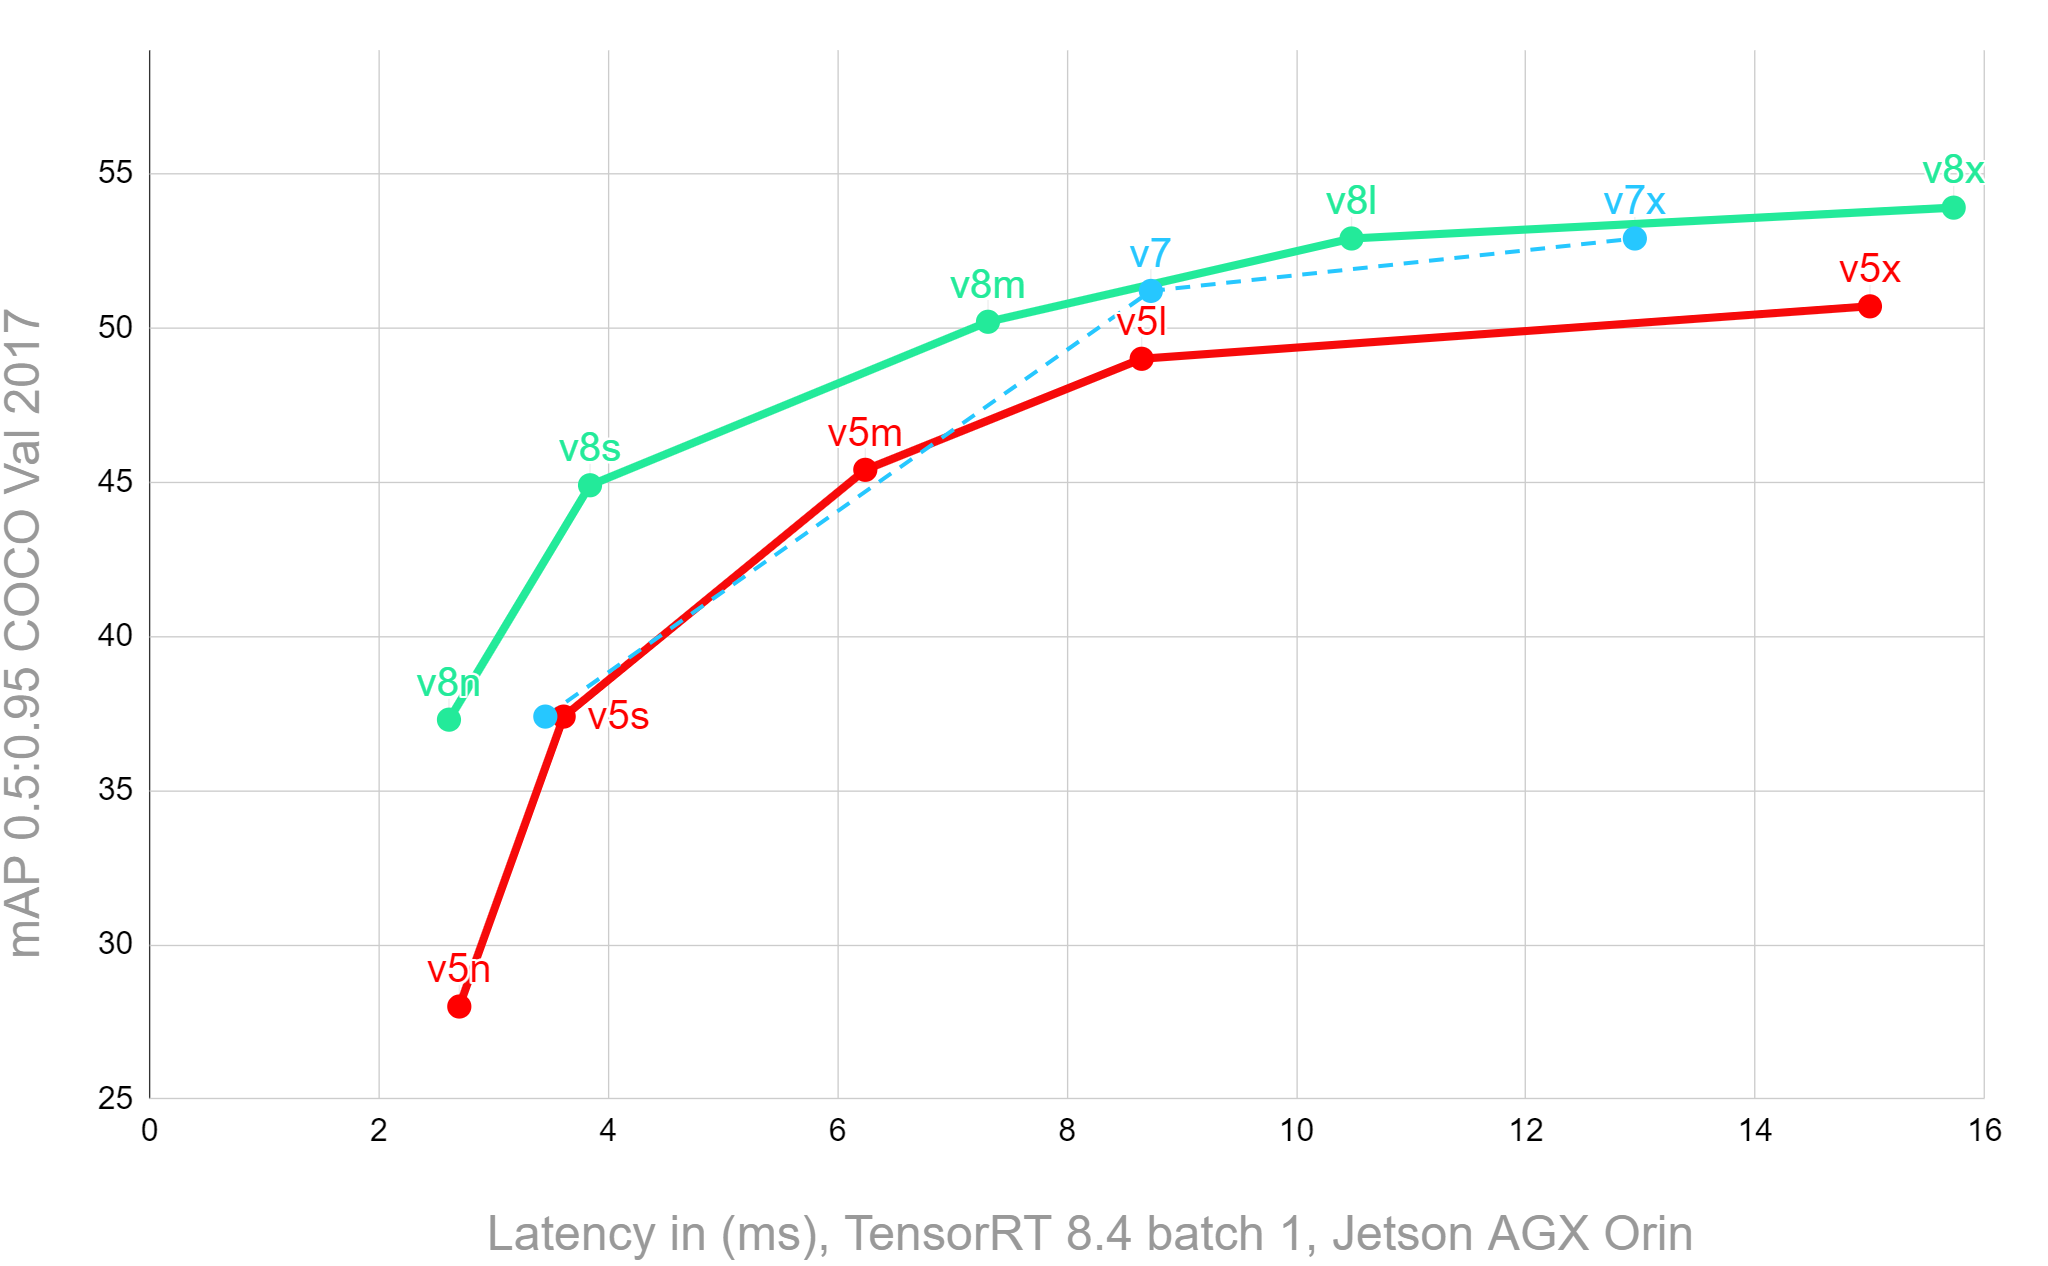
\includegraphics[width=10cm]{Images/YOLO Comparison Chart.png}
\caption{YOLO Comparison Plot \cite{deep9}}
\label{yolocomp}
\end{figure}

Although many researchers have developed and utilized many deep learning models for sperm detection, deep learning still has some drawbacks. Firstly, deep learning models require a lot of data and labeling labor to produce reliable detection results, which are often very expensive. Secondly, even the lightest models require computational resources, such as GPU support and large memory. However, deep learning's advantages make it a better choice for sperm detection. Deep learning models can learn complex and nonlinear features from the data. From the learning, the models can detect the sperm cells flexibly, detecting partially occluded sperms and sperms out of focus from the camera. Therefore, deep learning is still advantageous over traditional approaches.
\newpage
\section{Object Tracking}
Object tracking is a fundamental task in computer vision to locate and identify objects of interest in a video sequence. One main challenge is handling multiple objects simultaneously, especially when they have similar shapes and colors, undergo occlusion, and move unpredictably. Multiple object tracking (MOT) can be formulated as a data association problem, where the goal is to assign identification numbers to objects and build the movement tracks. There are two main categories of object tracking methods: online and offline. Online methods process the detections sequentially and update the tracks in each frame, while offline methods collect all the detections in a batch and optimize the tracks globally. As this project aims to build a real-time detection model, only the online models will be discussed further in this paper.

One of the most well-known online tracking models is Simple-Online-and-Realtime-Tracking (SORT) model built by Bewley et al. \cite{SORT} SORT utilized the Kalman filter to associate objects from different timesteps in sequential frames. The advantage of the Kalman filter in object tracking tasks is that it can predict the current position of an object based on the movement of the same object in previous frames. Moreover, due to its recursive nature, the Kalman filter does not take much space in memory and has a faster execution period, which makes it a favorable choice for real-time tracking tasks. Wojke et al. introduced deep learning techniques to the SORT algorithm, enhancing the original motion model with deep learning components that take account of the visual features of the detections to make better tracking. \cite{DeepSORT}

From many previous pieces of research about sperm tracking, the Kalman filter paired with the Hungarian assignment algorithm works well. From the works of Jati at el., the Kalman filter paired up with the Hungarian assignment algorithm worked well even in low frame rate videos. \cite{KalmanHungarian}
\chapter{Methodology}
In this chapter, the methodology of the project will be explained in detail, covering the following aspects: dataset generation, model selection, model training, and object tracking. The dataset generation section will describe how the training data was extracted from the video and split into train and test sets. The model selection section will justify the choice of the YOLOv8 model for object detection and compare it with its size variants. The model training section will present the steps in training the YOLOv8 model on the custom dataset, including hyperparameter tuning and validation. The object tracking section will introduce the algorithm for tracking detected objects across frames. 
\newpage
\section{Dataset Generation}
The first step in this project was to generate a dataset of sperm images from the videos provided by the supervising professor. The videos were uploaded to Roboflow, a platform for data scientists for data collection and annotation. Then, the video was converted to frames using their frame extract tools, with a rate of 5 frames per second, resulting in 1400 frames. 

The next step was to label the sperms in each frame using a bounding box annotation tool. Around the first 600 images were manually labeled by drawing a rectangle around each sperm and assigning their class as a sperm. Later images were aided by a deep learning model trained by the first part of the annotation task. The model would generate a preliminary annotation on the images, and the annotators only have the task of correcting the model's predictions and labeling unnoticed sperms, reducing the workload of annotators by a significant amount. 

\begin{figure}[h]
\centering
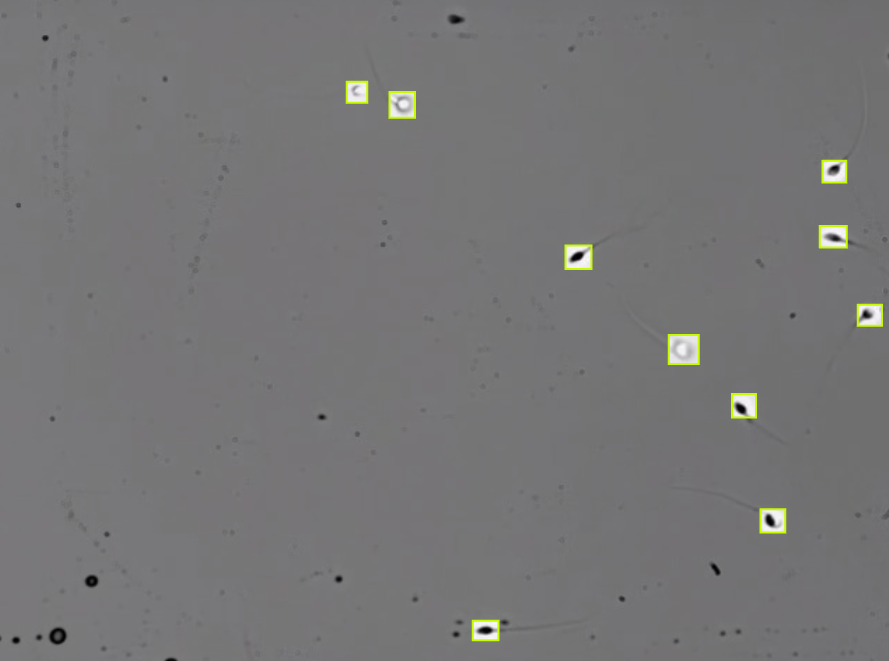
\includegraphics[width=0.85\textwidth]{Images/Labeled Frame.png}
\caption{Labeled Frame}
\end{figure}

After all 1400 images were annotated thoroughly, they underwent a full reinspection to find discrepancies in annotating rules and styles between earlier and later annotations. Although deep learning models generally can cope with such imperfections, it has been taken extra care to optimize the fitness and performance of the trained models.

\subsection{Train/Validation/Test Split}
Train/validation/test split is a technique that divides the data into three subsets: one for training the model, one for validating the model while training, and one for testing it. The training subset is used to fit the model parameters. It is crucial that the model only learns from the training set because it lowers the objective credibility of the model's performance. The validating subset measures the model's performance while training, usually after every epoch\footnote{One epoch means every image from the dataset has been fed to the training model and used to update the parameters once.} of training. The validation set gives an objective perspective of finding the optimal points to stop training from the training set to prevent the model from overfitting. Lastly, the testing subset is used to test the model with an entirely new set of data after training. Many hyperparameters can be tuned to enhance or degrade the model's performance, and test set images help compare models with different hyperparameters and find the best working setting for training. 

Although there is no golden ratio for the train/validation/test split, it is essential to set the test and validation sets to have adequate data to gain a meaningful assessment of the model. It is often misunderstood that a larger training set is always good for model performance. Still, to prevent the model from overfitting to the training set, there need to be some resources allocated to the validation and test set. For big projects with millions of training data, the testing and validation ratio can be as low as 1\%. Still, in this project, only with 1400 images, the ratio has to be significantly higher. For standard practices, according to Baheti from V7Labs, the most popular split choices for small-scale projects like this one are 60/20/20, 70/15/15, and 80/10/10. \cite{baheti} The three choices will be later examined in Subsection \ref{hyper}, as the split scheme is also part of major hyperparameters in training the model.

\subsection{Dataset Quality Analysis}
Examining the qualities of a dataset and addressing any issues is an essential process before training the model because training the model takes a lot of resources. If a dataset is poorly developed, it will affect the performance and credibility of the trained model. Usually, there are three considerations: class representations, annotation positions, and counts per frame. The first element can be neglected because this project only has one class, sperm. For the second element, Figure \ref{hitmap} is this dataset's hit map of annotations. Although there are a few hotspots, the sperms are generally well spread across the whole frame.
\newpage
\begin{figure}[ht]
\centering
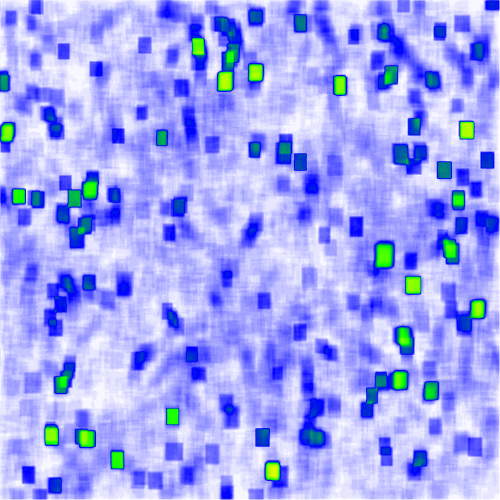
\includegraphics[width=9.6cm, height=7.2cm]{Images/hitmap.png}
\caption{Annotation Hitmap}
\label{hitmap}
\end{figure}

For the last element, Figure \ref{Hist} shows the histogram of sperm counts in all images. As most images have less than 25 sperms, the model might underperform in detecting sperms in images with more than 25 sperms. To address this issue, more images with more than 25 sperms have been allocated to the validation and test sets to find the model that works well in all environments. 

\begin{figure}[h!]
\centering
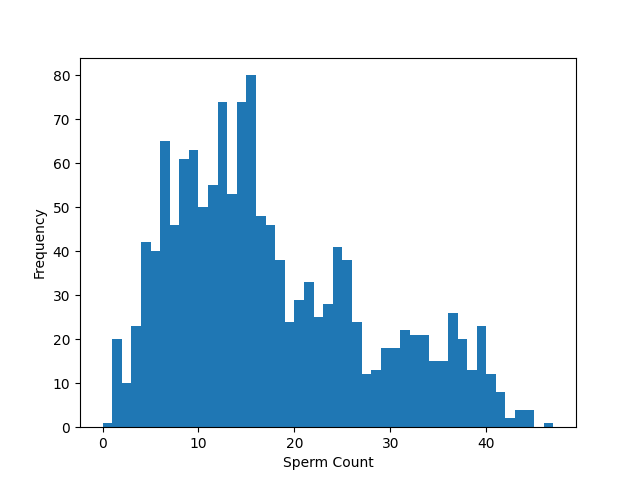
\includegraphics[width=11cm]{Images/Histogram.png}
\caption{Histogram of Sperm Counts}
\label{Hist}
\end{figure}

\subsection{Data Augmentation}
Data augmentation is a technique that can improve the performance and generalization of the trained model by increasing the size and diversity of the training data. The model learns to extract data from the image from a more diverse source of information, lowering the variance of the model. There are several data augmentation methods, but this project uses flipping, rotation, brightness, exposure, noise, and mosaic. For flipping, both horizontal and vertical flips were used, rotation was conducted within 15 degrees to both clockwise and anticlockwise, and up to 10\% brightness was added and subtracted from the images. For exposure, up to 5\% deviation was made from the original, and up to 2\% noise was added to the image. Lastly, the images were split into small parts and combined for the mosaic, which increases the model's performance in detecting small objects. The training images were tripled after data augmentation, and from some preliminary results, they have proven to increase the performance and decrease the variance of the model. 

\begin{figure}[h!]
  \begin{minipage}{\linewidth}
  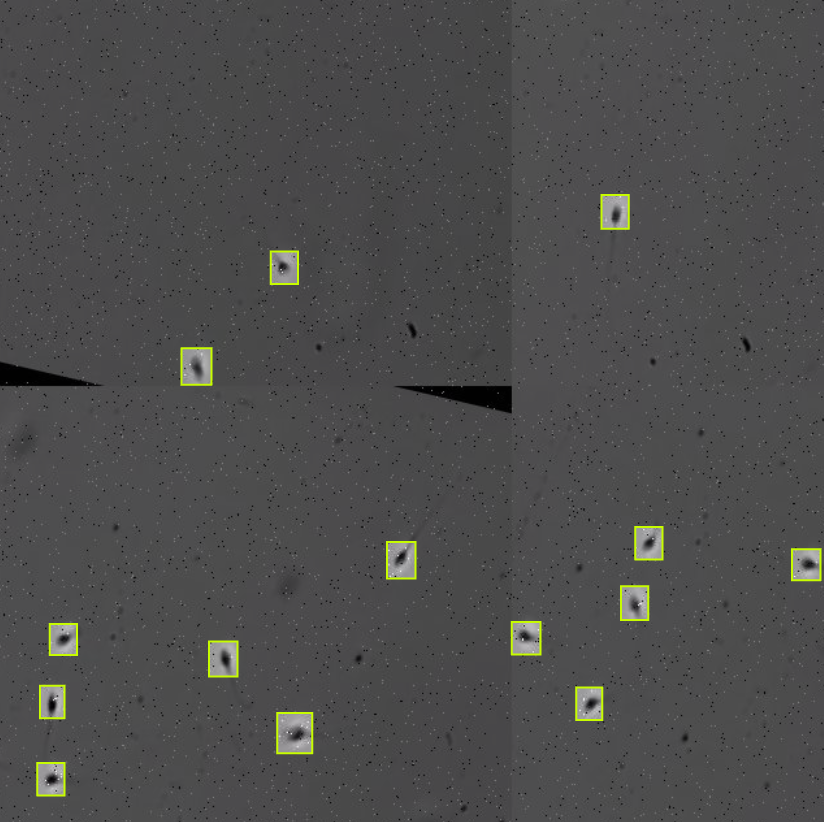
\includegraphics[width=.32\linewidth]{Images/aug1.png}\hfill
  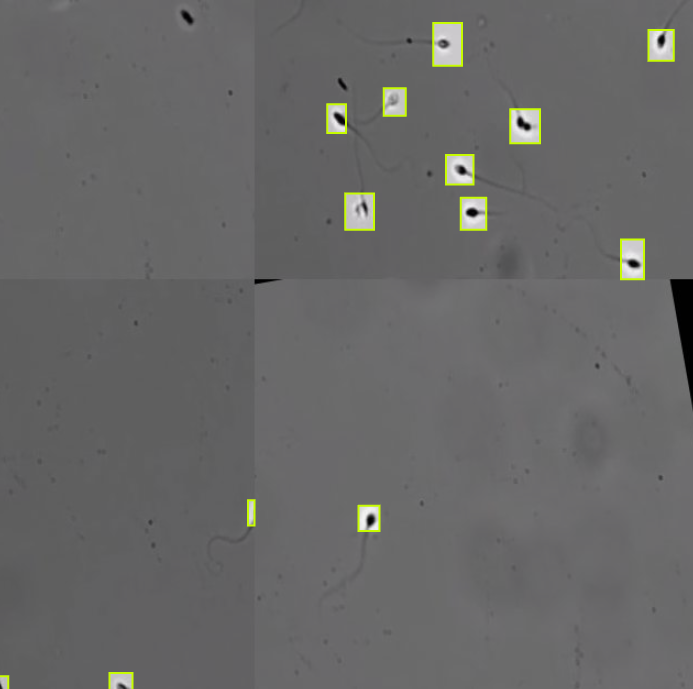
\includegraphics[width=.32\linewidth]{Images/aug2.png}\hfill
  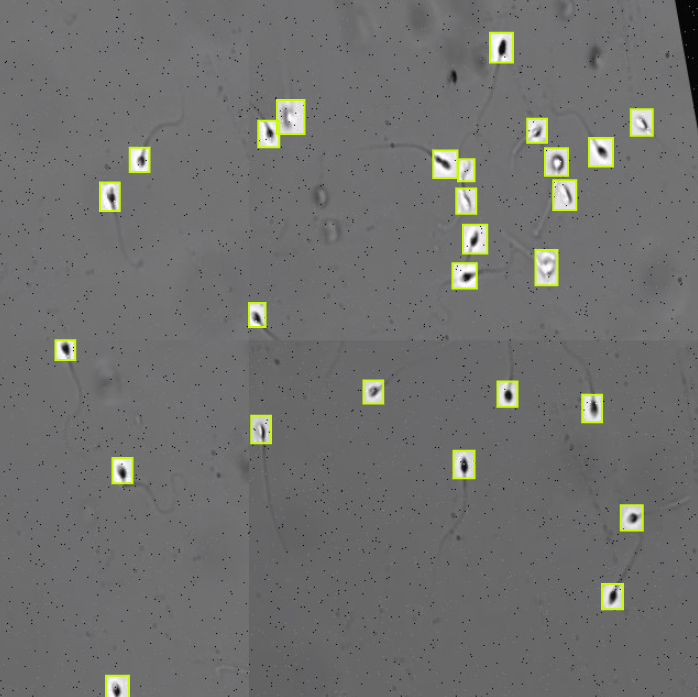
\includegraphics[width=.32\linewidth]{Images/aug3.png}%
  \end{minipage}%
  \caption{Examples of Augmented Images}
  \label{aug}
\end{figure}

\newpage
\section{Model Selection}
Model selection is an essential step in the methodology of any machine learning project, as it determines the accuracy and validity of the results. As described in Chapter \ref{lit}, YOLO models are the most popular models for object detection, and even in sperm detection tasks, many researchers have proven their effectiveness in detecting sperm cells. As many variant models exist in YOLO, it is very important to find which one to use. From the general understanding of the data science community, YOLOv5 and YOLOv8 are considered the most effective models, with excellent community support and user-friendly resources. As shown in Figure \ref{yolocomp}, because YOLOv8 had better performance at a similar latency rate, the project chose YOLOv8 for the detection model.

\subsection{Model Size}
YOLOv8 provides 5 model sizes: nano, small, medium, large, and x-large. Bigger models have more parameters and higher performance, but smaller models take a shorter time to train and have smaller latencies. Because there were insufficient computational resources, this project only tested three smaller models. Each model was trained for 25 epochs with the same training conditions, and the result is shown in Table \ref{yolotable}.

\begin{table}[ht]
\centering
\begin{tabular}{|l|c|c|c|c|c|}
\hline
Size   & mAP50 & mAP50-95 & \begin{tabular}[c]{@{}c@{}}Training Time\\ (seconds/epoch)\end{tabular} & \begin{tabular}[c]{@{}c@{}}Latency\\ (ms/frame)\end{tabular} & \begin{tabular}[c]{@{}c@{}}Model Size\\ (MB)\end{tabular} \\ \hline
Nano   & 0.960 & 0.515    & 105                                                                     & 10                                                           & 6.0                                                       \\ \hline
Small  & 0.972 & 0.531    & 115                                                                     & 21                                                           & 23.3                                                      \\ \hline
Medium & 0.976 & 0.584    & 125                                                                     & 38                                                           & 197.9                                                     \\ \hline
\end{tabular}
\caption{Comparison of YOLOv8 Models}Training GPU: Tesla T4, Latency GPU: GTX 1660 Super
\label{yolotable}
\end{table}

For the accuracy of the models, a specific standard for object detection tasks was used. mAP stands for mean average precision, and for mAP50, the intersection over union (IOU) threshold was 50\%. The nano model has a performance of about 96\% of the detections made by the model had 50\% or more IOU with the ground truth. The IOUs of detections are calculated in Figure \ref{iou}. mAP50-95 is the weighted average for all mAPs over 50\% to 95\%.

\newpage

\begin{figure}[ht]
\centering
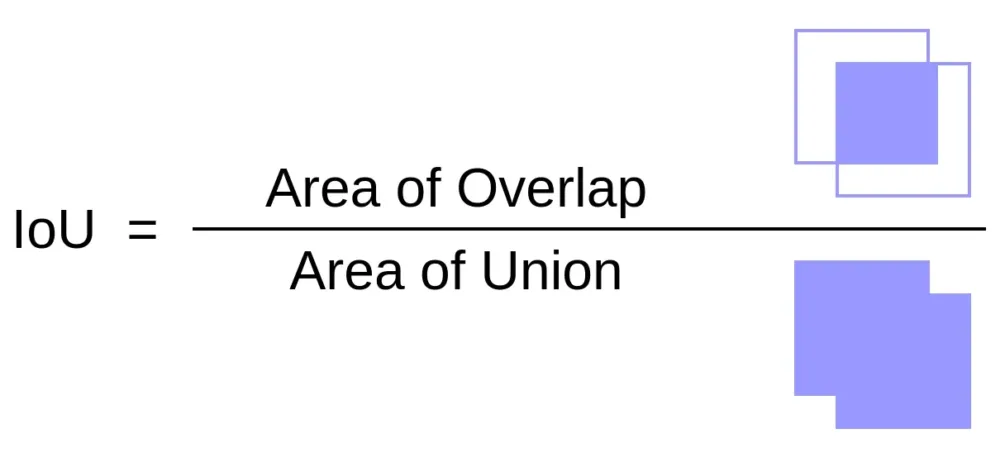
\includegraphics[width=13cm]{Images/iou.png}
\caption{IOU Calculation Method \cite{iou}}
\label{iou}
\end{figure}

From Table\ref{yolotable}, it can be seen that even the nano-sized model is performing well. However, it is still noticeable that the gap between nano and small models is quite large. Although the medium-sized model performed the best, the latency measured with the provided GPU was still too high to be used in a real-time tracking model. Therefore, the small-sized model was chosen to be used in this project. 

\newpage
\section{Model Training}
This section will explain how the model was trained. The model training process consists of three main steps: environment setup, hyperparameter tuning, and validation. The hardware and software requirements and the libraries and frameworks used for implementing the model will be explained in the environment setup step. In the hyperparameter tuning step, the methods and criteria for selecting the optimal values of the model parameters, such as learning rate, batch size, number of epochs, etc., will be discussed. The validation step will discuss how the models are tested with a held-out test set and validated.

\subsection{Environment Setup}
Like many machine learning projects, Python language was used in this project. To download and install YOLOv8, one can use Python's built-in package installer, pip. Several other libraries need to be installed together, which will be automatically detected by the installer and installed together. 
\begin{verbatim}
    pip3 install ultralytics
\end{verbatim}
The above line should be run at the Command Prompt. It is always better to download and install libraries in a virtual environment to prevent collisions. The above line should install almost all packages and libraries for this project. Still, for the remaining packages, if any, one can find \verb|requirements.txt| at \href{https://github.com/rladntjr7/FYP}{\underline{GitHub}} and run the following line at Command Prompt.
\begin{verbatim}
    pip3 install -r requirements.txt
\end{verbatim}

GPU support comes in handy for training and predicting with machine learning models. GPU parallel computing is a lot faster than CPU. Depending on the model, the GPU is 20 \~{} 100 times faster than the CPU. For training, Google Colab, a Cloud GPU provider, was used. GTX 1660 super was used as this project's primary computation unit for any other applications. Moreover, the CUDA framework from NVIDIA also needs to be installed for GPU involvement in model training. 
\newpage
\subsection{Hyperparameter Tuning}\label{hyper}
Many hyperparameters can be tuned to increase the model performance. Finding the optimal setup includes a lot of guesswork, and every project needs a different setup, so it is challenging to refer to others' work. However, there is a general guideline in the machine learning community written by AI engineers from Google, and it is called Deep Learning Tuning Playbook. \cite{tuningplaybookgithub} 

From the playbook, some important prerequisites need to be set before tuning the model:
\begin{itemize}
    \item Dataset is well organized.
    \item The environment is well prepared to minimize the time spent on the execution of training and validation of the model.
    \item The metric for analyzing the performance of the model is selected.
\end{itemize}

From the works from the previous sections, the first two items are already assessed. The main criteria for assessing the model will be mAP50, as the model does not require a very high precision due to the presence of the Kalman filter in the tracking stage. 

To increase the training throughput, a larger batch size\footnote{Batch size governs the number of training samples the model trains before updating the model's parameters. A larger batch size is advantageous because it decreases the number of steps within an epoch.} was used to expedite the training process. A higher training throughput will lead to a faster optimization of the model. The ideal batch size is usually the biggest size that the hardware can handle. From some experiments, the largest batch size available from Google Colab's Tesla T4 GPU is 42, and it decreased the training time by 30 seconds per epoch for the small-sized model. To further increase the speed, A100 GPU was used from the premium version of Google Colab, and it decreased the training time to around 15 seconds per epoch by using a batch size of 142. 

Some of the first things to consider were the dataset split and optimizer. As introduced earlier in this report, three splits will be tested, 60/20/20, 70/15/15, and 80/10/10. Four optimizers are available with YOLOv8: SGD, Adam, AdamW, and RMSProp. First, the data split will be tested by training the model for 20 epochs for each split. The result is displayed in Table \ref{splittable}.

\newpage

\begin{table}[h]
\centering
\begin{adjustbox}{max width=\textwidth}
\begin{tabular}{|c|cc|cc|cc|cc|}
\hline
\multirow{2}{*}{\textbf{Split}} & \multicolumn{2}{c|}{\textbf{Trial 1}}                                                                                                        & \multicolumn{2}{c|}{\textbf{Trial 2}}                                                                                                        & \multicolumn{2}{c|}{\textbf{Trial 3}}                                                                                                        & \multicolumn{2}{c|}{\textbf{Average}}                                                                                                        \\ \cline{2-9} 
                                & \multicolumn{1}{c|}{\begin{tabular}[c]{@{}c@{}}Validation\\ Accuracy\end{tabular}} & \begin{tabular}[c]{@{}c@{}}Test\\ Accuracy\end{tabular} & \multicolumn{1}{c|}{\begin{tabular}[c]{@{}c@{}}Validation\\ Accuracy\end{tabular}} & \begin{tabular}[c]{@{}c@{}}Test\\ Accuracy\end{tabular} & \multicolumn{1}{c|}{\begin{tabular}[c]{@{}c@{}}Validation\\ Accuracy\end{tabular}} & \begin{tabular}[c]{@{}c@{}}Test\\ Accuracy\end{tabular} & \multicolumn{1}{c|}{\begin{tabular}[c]{@{}c@{}}Validation\\ Accuracy\end{tabular}} & \begin{tabular}[c]{@{}c@{}}Test\\ Accuracy\end{tabular} \\ \hline
60/20/20                        & \multicolumn{1}{c|}{96.8\%}                                                        & 96.2\%                                                  & \multicolumn{1}{c|}{96.4\%}                                                        & 95.6\%                                                  & \multicolumn{1}{c|}{96.8\%}                                                        & 96.2\%                                                  & \multicolumn{1}{c|}{96.7\%}                                                        & 96.0\%                                                  \\ \hline
70/15/15                        & \multicolumn{1}{c|}{97.6\%}                                                        & 95.1\%                                                  & \multicolumn{1}{c|}{97.6\%}                                                        & 95.1\%                                                  & \multicolumn{1}{c|}{97.6\%}                                                        & 94.0\%                                                  & \multicolumn{1}{c|}{97.6\%}                                                        & 94.7\%                                                  \\ \hline
80/10/10                        & \multicolumn{1}{c|}{97.9\%}                                                        & 95.9\%                                                  & \multicolumn{1}{c|}{97.7\%}                                                        & 95.4\%                                                  & \multicolumn{1}{c|}{97.7\%}                                                        & 95.4\%                                                  & \multicolumn{1}{c|}{97.8\%}                                                        & 95.6\%                                                  \\ \hline
\end{tabular}
\end{adjustbox}
\caption{Comparison of Different Dataset Split}Metric: mAP50
\label{splittable}
\end{table}

In Table \ref{splittable}, three trials were conducted for each split, and the average accuracies were shown in the last two columns. Of all splits, the 70/15/15 split performed the worst. Presumably, the 60/20/20 split benefitted the model with the testing performance from the larger validation set, and the 80/10/10 split had a greater fit to the data with the larger training set. 

Although the 80/10/10 split performed the best in validation, its testing accuracy was lower than 60/20/20. Because testing accuracy is the most important criterion and with the lowest variance, the 60/20/20 split was selected for this project. 

The next step is choosing the optimizer. From the above four options, SGD\footnote{Stochastic Gradient Descent} is the most basic option, where the parameters are updated from a few random samples from the batch. SGD is fast because the model does not have to learn from all training samples within the batch. However, because optimization is a global minimum problem in a multi-dimensional space, SGD's inability to escape from local minima quickly is a critical disadvantage. The other three optimizers try to mitigate this issue using different techniques. RMSProp uses the moving average of gradients and reduces the oscillation of weights by dividing the moving averaged gradient by the gradient's root mean square (RMS). On the other hand, Adam combines RMSProp with the concept of momentum, where the gradient is less likely to be reduced when the history of gradients has a similar direction. AdamW involves weight decay, increasing the convergence rate and the generalization of the model. 

For many cases, AdamW is the optimal choice, and many indicate that using AdamW is not degrading the model's performance in most cases while reducing overfitting.\cite{adamw} Therefore, AdamW will be the main optimizer for training in this project. Other optimizers will be assessed as well if AdamW underperforms significantly. 
\newpage
The learning rate has to be scheduled for the last step before training the model. Learning rates are significant in training because if the rate is too low, the model will not gain any updates from the training. If the rate is too high, the gradients will make the model oscillate, making it harder to reach the global minimum or even diverge. 

This project uses the pre-trained model by the makers of YOLOv8. The original model was trained from the COCO dataset. \cite{coco} Because the weights in earlier layers are already optimized to find specific characteristics from the images, the learning rate has to be kept low. Three learning rates will be tested to find the optimal training setting, which will be 0.001 as the original setting, 0.0005, and 0.0001. Figure \ref{lrcomp} shows the effect of different learning rates on the training loss.

\begin{figure}[h]
    \centering
    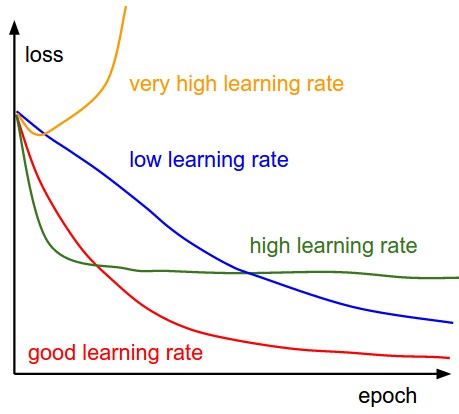
\includegraphics[width = .8\textwidth]{Images/learning rate.jpeg}
    \caption{Learning Rate Comparison \cite{cs231n}}
    \label{lrcomp}
\end{figure}

\newpage
The three learning rates were tested with 50 epochs each, and Figure \ref{lrtest} shows the effect of the learning rate on training losses. 

\begin{figure}[h]
  \begin{minipage}{\linewidth}
  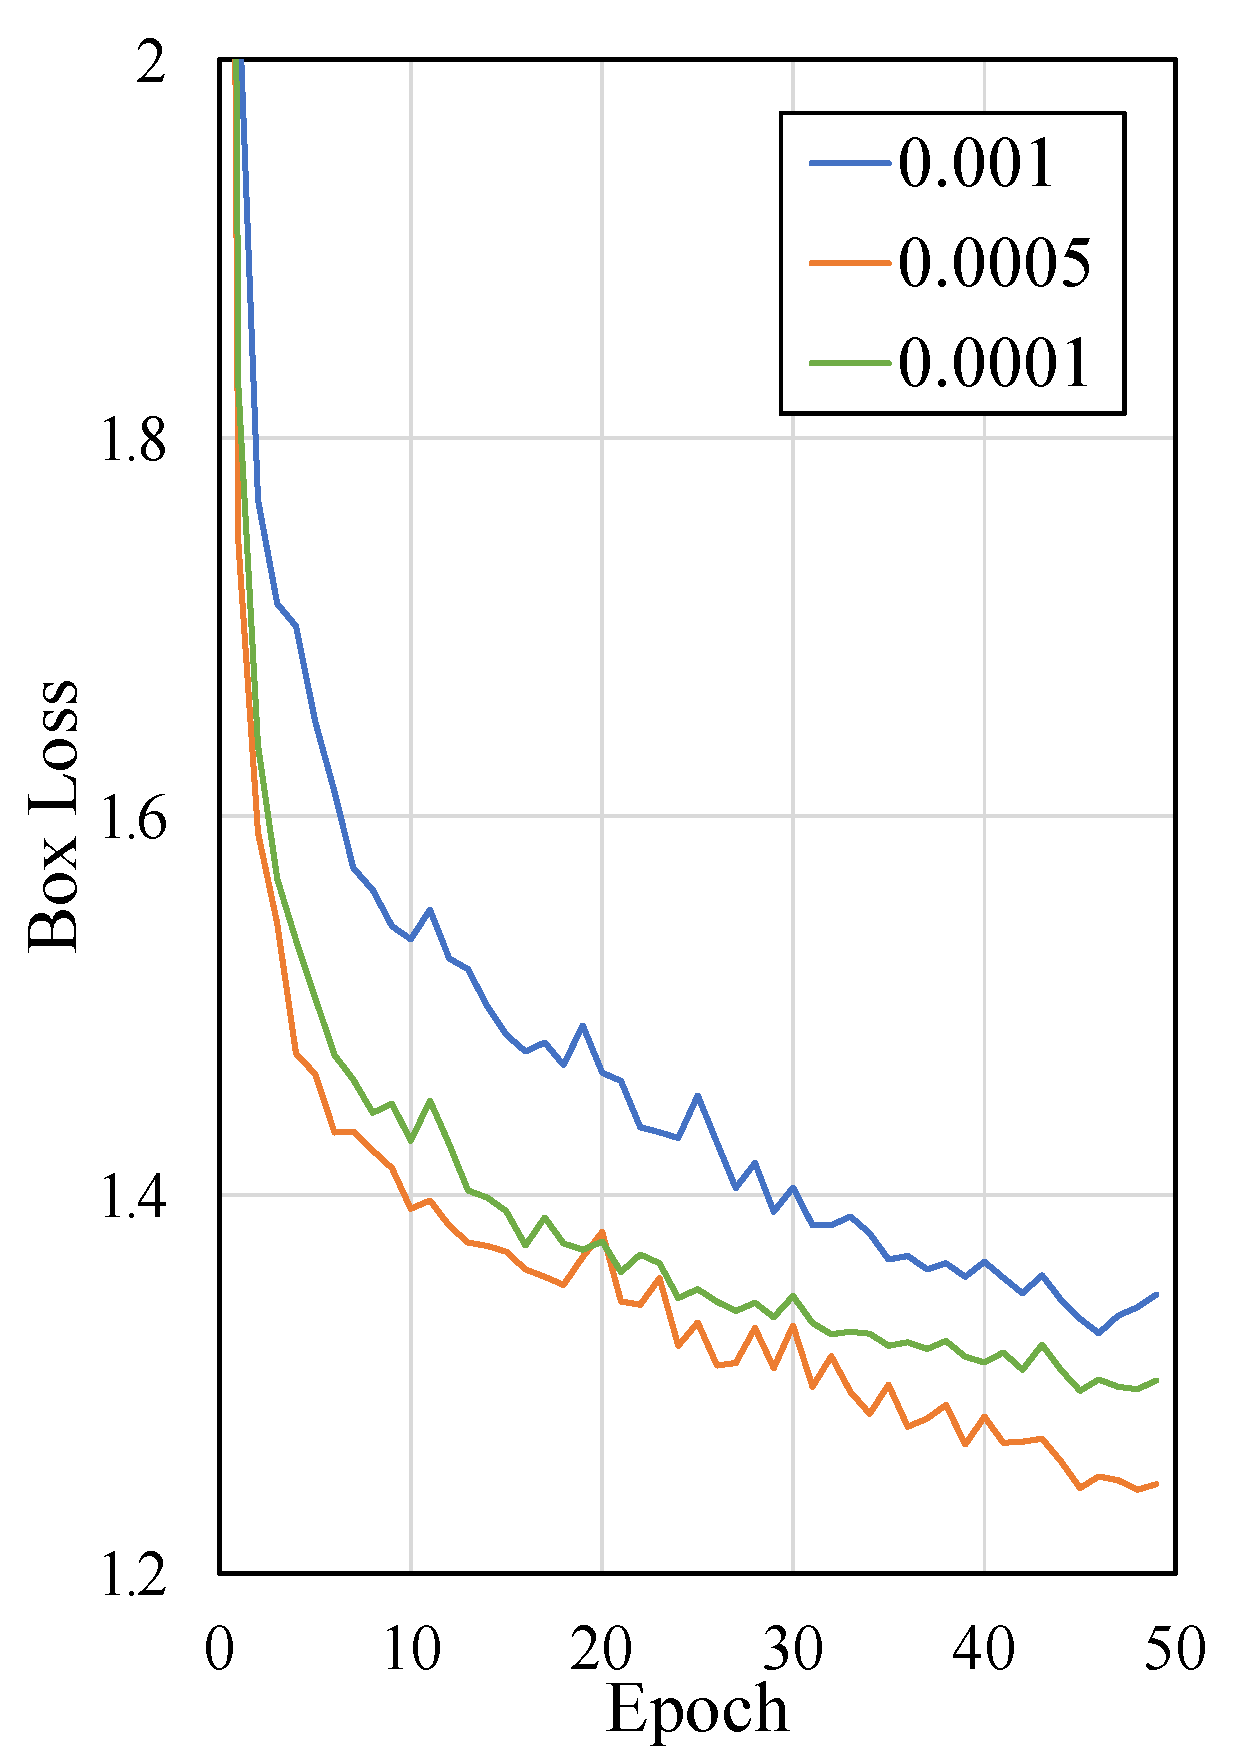
\includegraphics[width=0.33\linewidth]{Images/box loss.pdf}\hfill
  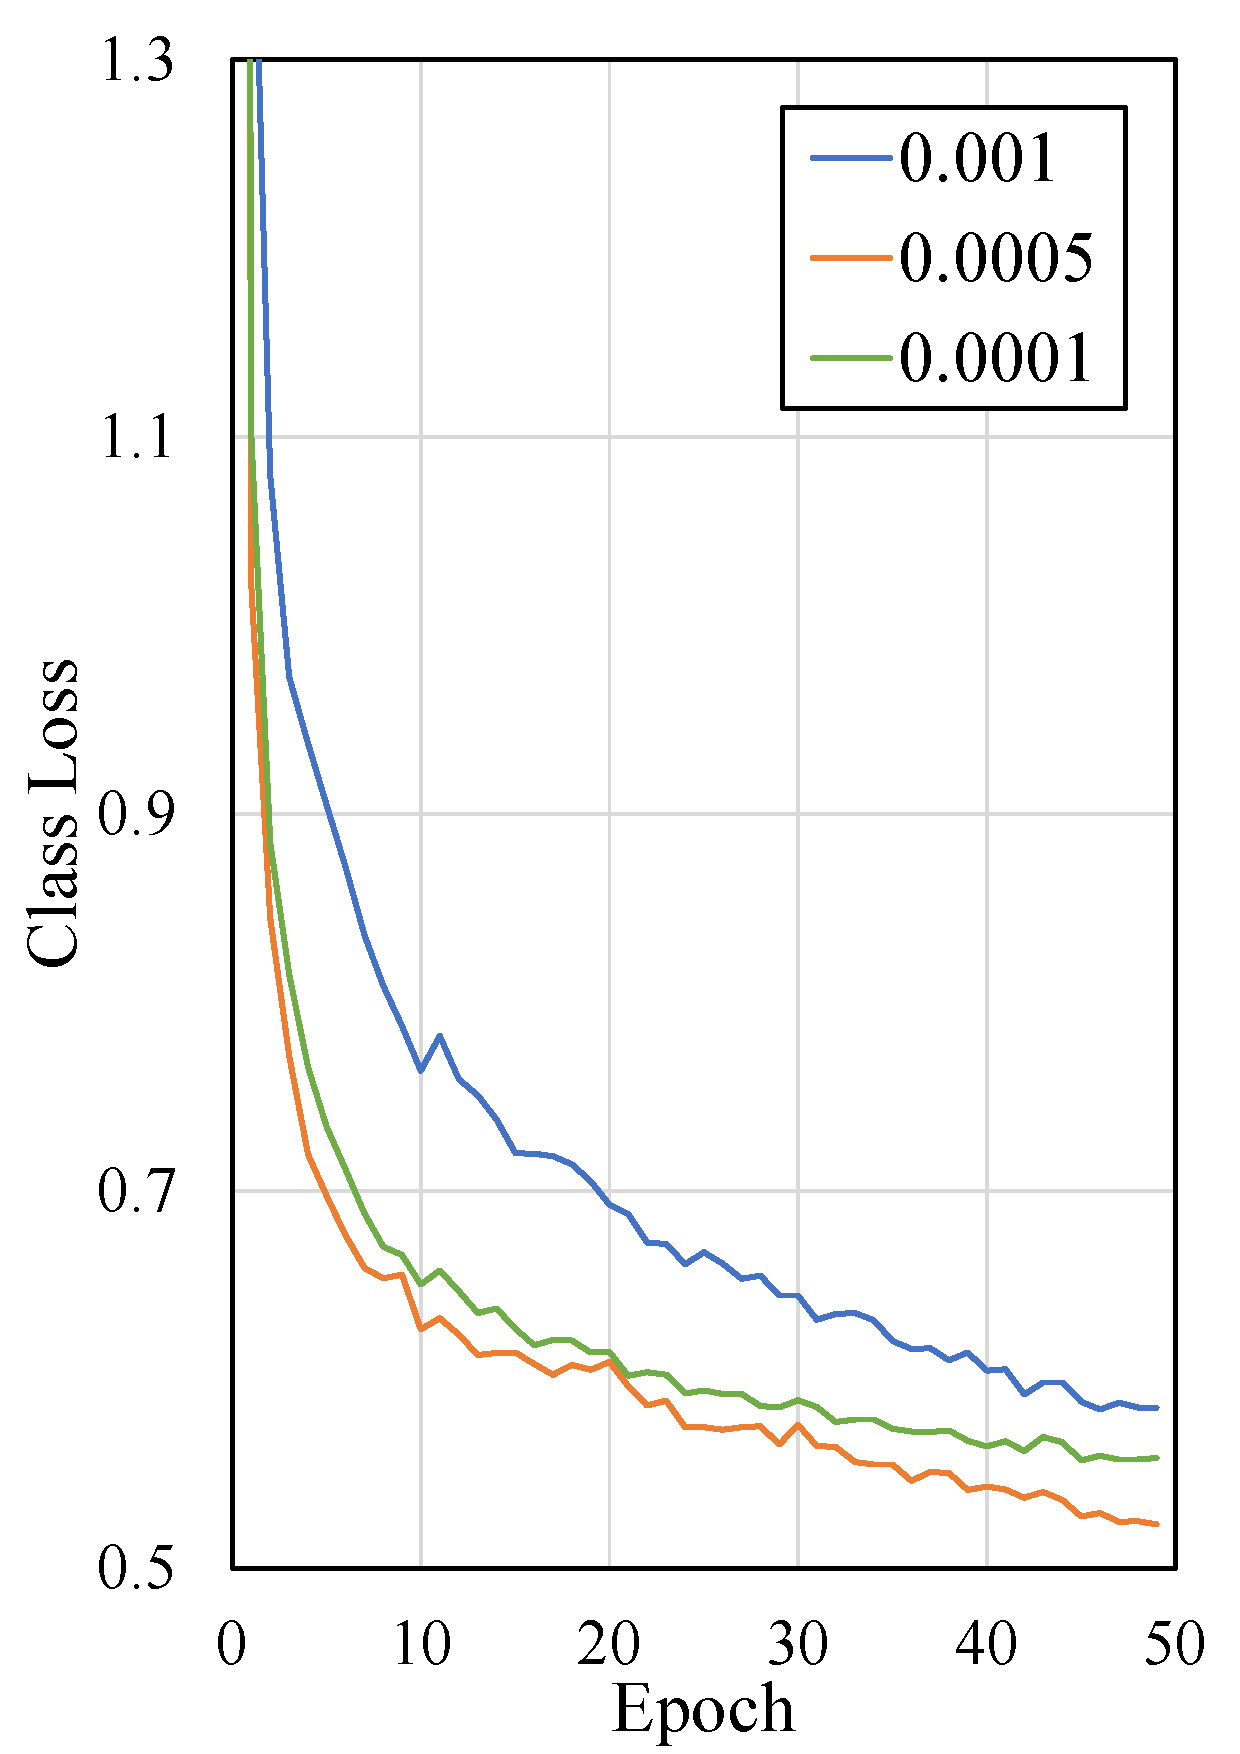
\includegraphics[width=0.33\linewidth]{Images/class loss.pdf}\hfill
  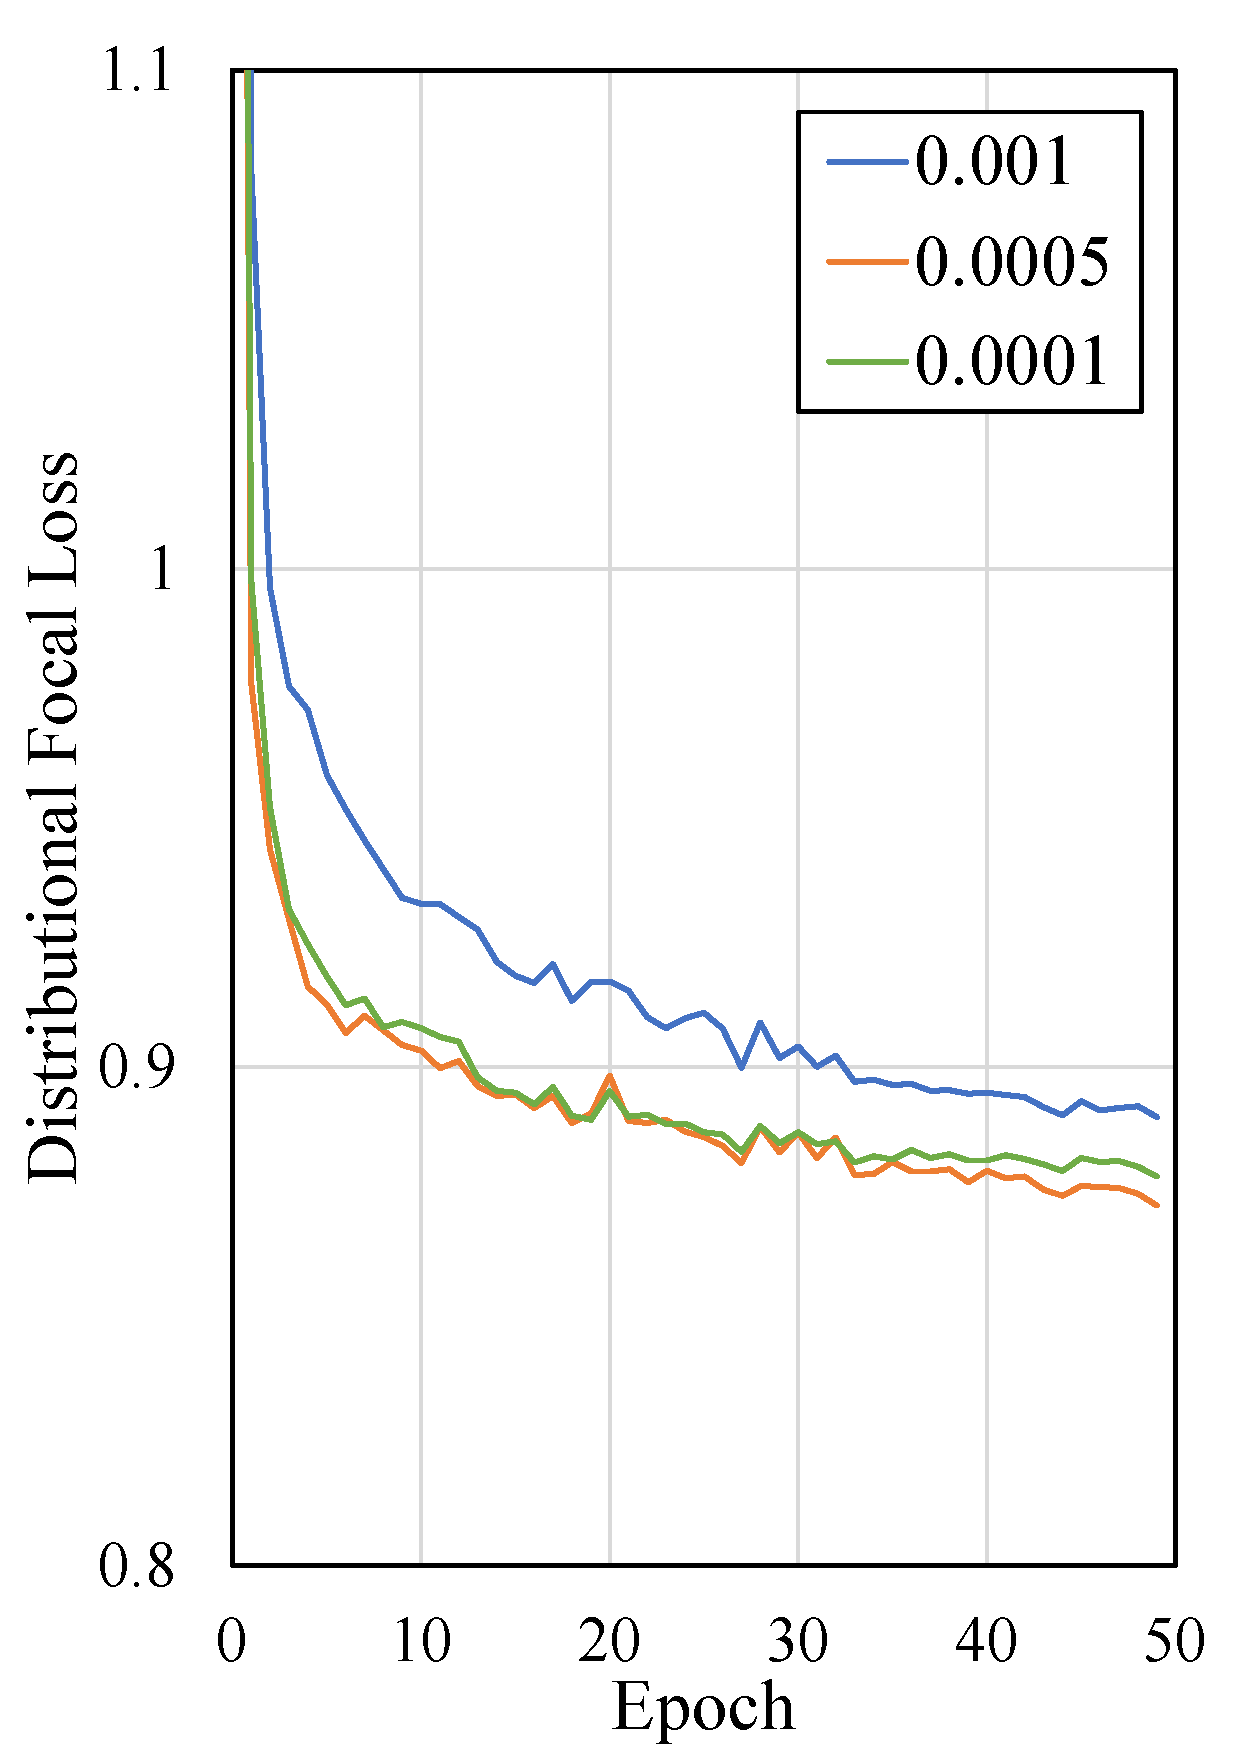
\includegraphics[width=0.33\linewidth]{Images/dfl loss.pdf}%
  \end{minipage}%
  \caption{Learning Rate Test Result}
  \label{lrtest}
\end{figure}

When the results are compared with Figure \ref{lrcomp}, the 0.001 learning rate seems to be too high, and the 0.0001 rate is too low. It can be found that the learning rate of 0.0005 is the adequate learning rate for this project. Although 54 hyperparameters can be tuned for the training of a YOLOv8 model, most of them are already optimized for general training and are not as important as the ones tuned explicitly in this project. Moreover, due to the limitation of computational resources, hyperparameter tuning will be finalized at this stage. 

\subsection{Validation}
Model validation evaluates the model's performance if it has reached the target and can be used for the intended purpose. Model validation is an essential step in any machine learning project. It helps ensure that the model is not overfitting or underfitting to the data and generalizing well to unseen scenarios. After training the model with finalized settings for 100 epochs, the model will be evaluated in Chapter \ref{results}, using various metrics and plots, such as accuracy, precision, recall, F1-score, etc.

\newpage
\section{Object Tracking}
This section will explain what methods were used in the tracking part of the project. Object tracking of sperm cells is difficult because they do not always move consistently, often becoming out of focus and undetected by the model. This project managed to keep track of most sperms in the frames, and the primary method is shown as the flow chart in Figure \ref{flowchart}.

To facilitate the tracking of sperm, a sperm class was made under \verb|sperm.py|, where the sperm needs an identification number and the coordinates of the bounding box for declaration. The class's \verb|__init__| function assigns various attribute elements for tracking, including many matrices for the Kalman filter and activity indexes. Detailed analysis of the tracking algorithm will be described in the following subsections. 

\clearpage
\begin{figure}[ht!]
\centering
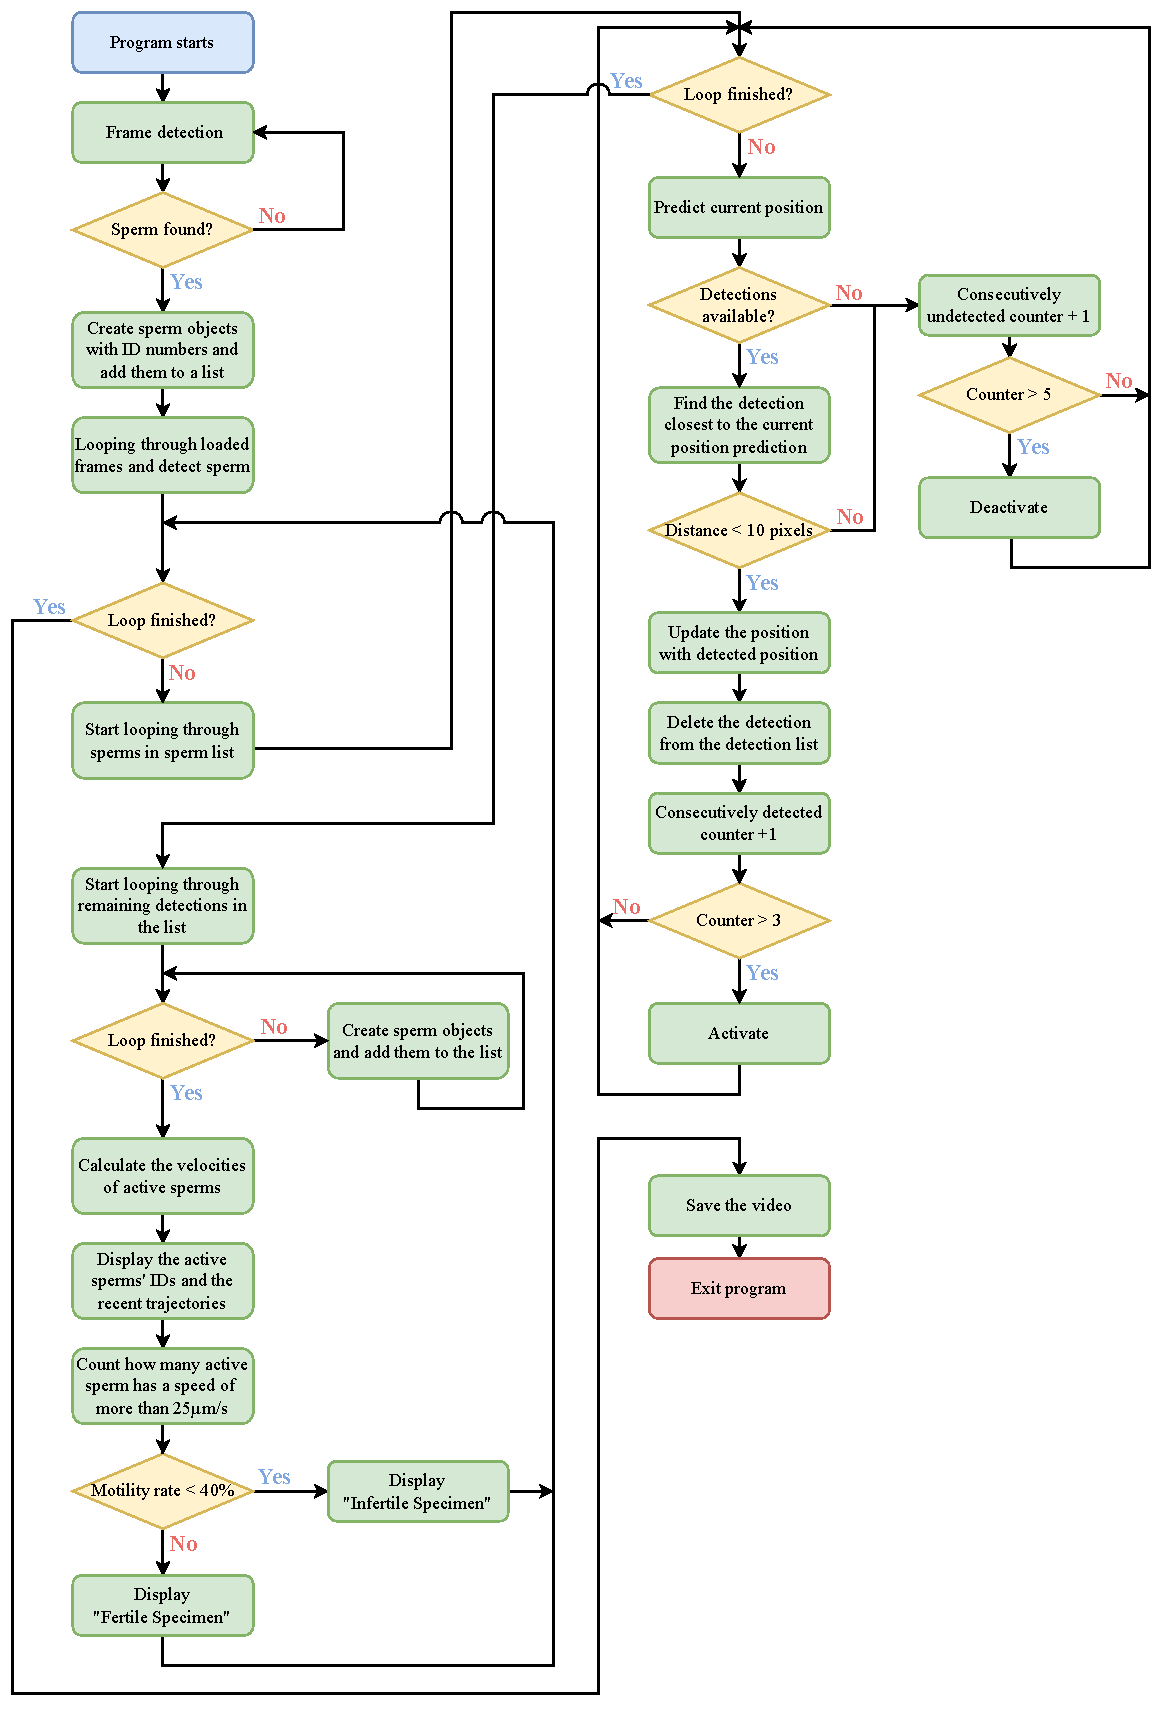
\includegraphics[width=13cm]{Images/flowchart.drawio.pdf}
\caption{Flowchart of the Program}
\label{flowchart}
\end{figure}


\subsection{Kalman Filter} \label{kalman}
Kalman filters, usually called noise filters, find optimal state estimations based on uncertain measurements and predictions. \cite{kalman}\cite{kalman2} Kalman filters are used anywhere an accurate status estimation is needed, including GPS, Radar, economics, etc. Object tracking systems also require optimal estimations to track the objects smoothly, even if they are occluded or blurry. Kalman filter is especially very useful in this project because, from its recursive nature, the Kalman filter only uses a minimal amount of memory, which is very useful when sometimes there are hundreds of items to track throughout the whole video. 

The basic equations of the Kalman filters are Equations \ref{kal1} and \ref{kal2}. 
\begin{equation} \label{kal1}
    X_k = AX_{k-1} + Bu_{k-1}+w_{k-1}
\end{equation}
\begin{equation} \label{kal2}
    Z_k = HX_k + v_k
\end{equation}
where Equation \ref{kal1} is the prediction equation of the Kalman filter from the previous information about an object. Equation \ref{kal2} represents the current measured status. \(w_k\) and \(v_k\) represent the noises from the prediction and measurement, and they are assumed to be following the Gaussian distribution with covariance matrices \(Q\) and \(R\), respectively.

The following kinematic equations were set up to derive the components for Equation \ref{kal1}.
\begin{equation} \label{xcoor}
x_k=x_{k-1}+\Dot{x}_{k-1}\Delta t + \frac{1}{2}\Ddot{x}_{k-1}\Delta t ^2
\end{equation}
\begin{equation} \label{xvel}
\Dot{x}_k=\Dot{x}_{k-1}+\Ddot{x}_{k-1}\Delta t
\end{equation}

Equations \ref{xcoor} and \ref{xvel} can be simplified to a single matrix, 
\begin{equation} \label{xmat}
X_k = \begin{bmatrix} x_k \\ \Dot{x}_k\end{bmatrix}=\begin{bmatrix}
    x_{k-1}+\Dot{x}_{k-1}\Delta t + \frac{1}{2}\Ddot{x}_{k-1}\Delta t ^2 \\
    \Dot{x}_{k-1}+\Ddot{x}_{k-1}\Delta t
\end{bmatrix}
\end{equation}

Equation \ref{xmat} can be further simplified to matrix multiplication,
\begin{equation} \label{xmatsimp}
X_k = \begin{bmatrix} x_k \\ \Dot{x}_k\end{bmatrix} = \begin{bmatrix}
    1 & \Delta t \\
    0 & 1
\end{bmatrix}
X_{k-1}
+
\begin{bmatrix}
    \frac{\Delta t^2}{2} \\
    \Delta t
\end{bmatrix}
\Ddot{x}_{k-1}
\end{equation}

For the two-dimensional version of Equation \ref{xmatsimp},
\begin{equation} \label{xymat}
X_k = 
\begin{bmatrix} 
x_k \\ 
y_k \\ 
\Dot{x}_k \\ 
\Dot{y}_k
\end{bmatrix} 
= 
\begin{bmatrix}
    1 & 0 & \Delta t & 0 \\
    0 & 1 & 0 & \Delta t \\
    0 & 0 & 1 & 0 \\
    0 & 0 & 0 & 1
\end{bmatrix}
X_{k-1}
+
\begin{bmatrix}
    \frac{\Delta t^2}{2} & 0 \\
    0 & \frac{\Delta t^2}{2} \\
    \Delta t & 0 \\
    0 & \Delta t
\end{bmatrix}
\alpha _{k-1}
\end{equation}
where \(\alpha_{k}\) is a matrix of accelerations at time \(k\).

The two matrices of Equation \ref{xymat} are \(A\) and \(B\) from Equation \ref{kal1}.
\begin{equation}
    A = \begin{bmatrix}
        1 & 0 & \Delta t & 0 \\
        0 & 1 & 0 & \Delta t \\
        0 & 0 & 1 & 0 \\
        0 & 0 & 0 & 1
    \end{bmatrix}
    B = \begin{bmatrix}
        \frac{\Delta t^2}{2} & 0 \\
        0 & \frac{\Delta t^2}{2} \\
        \Delta t & 0 \\
        0 & \Delta t
    \end{bmatrix}
\end{equation}

The process noise covariance matrix \(Q\) can be defined as follows:
\begin{equation} \label{covQ}
Q = 
\begin{bmatrix}
    \sigma ^2_x & 0 & \sigma_x \sigma_{\Dot{x}} & 0 \\
    0 & \sigma ^2_y & 0 & \sigma_y \sigma_{\Dot{y}} \\
    \sigma_x \sigma_{\Dot{x}} & 0 & \sigma ^2_{\Dot{x}} & 0 \\
    0 & \sigma_y \sigma_{\Dot{y}} & 0 & \sigma ^2_{\Dot{y}}
\end{bmatrix}
\end{equation}
where it is assumed that there is no correlation between the two axes. 
The equation can be further simplified when the standard deviations of position and velocities are assumed to be \(\frac{\Delta t^2}{2}\sigma_a\) and \(\Delta t \sigma_a\), respectively, where \(\sigma_a\) is the standard deviation of the acceleration, and \(\Delta t\) is the time between timesteps. 

The process noise covariance matrix is now simplified as follows:
\begin{equation} \label{covQsimp}
Q = 
\begin{bmatrix}
    \frac{\Delta t^4}{4} & 0 & \frac{\Delta t^3}{2} & 0 \\
    0 & \frac{\Delta t^4}{4} & 0 & \frac{\Delta t^3}{2} \\
    \frac{\Delta t^3}{2} & 0 & \Delta t^2 & 0 \\
    0 & \frac{\Delta t^3}{2} & 0 & \Delta t^2
\end{bmatrix}
\sigma_a^2
\end{equation}

The transformation matrix \(H\) from Equation \ref{kal2} is defined as:
\begin{equation} \label{transmat}
H = 
\begin{bmatrix}
    1 & 0 & 0 & 0 \\
    0 & 1 & 0 & 0
\end{bmatrix}
\end{equation}
In this project, only the positions are measured by the detection model. Therefore, the velocity components are neglected. 

The measurement noise covariance matrix is defined as:
\begin{equation} \label{noiscov}
R = 
\begin{bmatrix}
\sigma_x^2 & 0 \\
0 & \sigma_y^2
\end{bmatrix}
\end{equation}
where the detection model is assumed that there are no dependencies between two coordinates during detections.

Moreover, it can also be assumed that the standard deviations of both coordinates are similar to each other, and the Equation \ref{noiscov} can be simplified as:
\begin{equation}
    \label{noiscovsimp}
    R=
    \begin{bmatrix}
        \sigma_m^2 & 0 \\
        0 & \sigma_m^2
    \end{bmatrix}
\end{equation}
where \(\sigma_m^2\) is the standard deviation of measurement in both axis. 

\subsubsection{Prediction}
A priori state (before status is updated with the measurement) is estimated with the following equation to predict the current status based on previous information.
\begin{equation}
    \label{priori}
    \hat{X}_k^- = A\hat{X}_{k-1} + B u_{k-1}
\end{equation}
where \(\hat{X}_k^-\) is the priori state estimate, and \(\hat{X}_{k-1}\) is the posteriori state estimate (after update with the measurement) from the last timestep \(k-1\). 

The priori error covariance matrix is calculated as follows:
\begin{equation}
    \label{prioricov}
    P^-_k = AP_{k-1}A^T + Q
\end{equation}
where \(P^-_k\) is the priori error covariance matrix, and \(P_{k-1}\) is the posteriori error covariance matrix from the last timestep.

\subsubsection{Update}
As the first step of the update stage, the Kalman gain \(K_k\) is calculated as the following equation.
\begin{equation}
    K_k=P^-_k H^T (HP^-_kH^T+R)^{-1}
\end{equation}
To update the prior state estimate to the posteriori state estimate, it has to be added by the product of the Kalman gain \(K_k\) and the measurement residual. The measurement residual is the difference between the current measurement and the previous estimation. Therefore it is \(Z_k - H\hat{x}^-_k\). So, the posteriori state estimate is calculated as follows: 
\begin{equation}
    \hat{X}_k = \hat{X}_k^- + K_k(Z_k - H\hat{x}^-_k)
\end{equation}

Also, the error covariance matrix \(P_k\) is updated, which will be used in the next timestep. 
\begin{equation}
    P_k = (I-K_h H)P^-_k
\end{equation}

\subsection{Tracking Algorithm}
This subsection will explain the tracking algorithm of this program in detail, including the utilization of the Kalman filter as defined in Subsection \ref{kalman}.

When the program starts, it brings the video and the detection model. The first frame is detected, and each detection is given an identification number and stored inside the \verb|sperm_list|. If there is no sperm in the first frame, the program loops until there is any sperm found. When the sperm is declared, all the Kalman filter components are initialized with the input parameters. 

Afterward, the program loops through the following frames in the video. For each frame, the program loops through the sperms in the \verb|sperm_list| and predicts the priori estimates with the \verb|predict()| function. For each sperm, it is checked if any detections are available in the detection list, and if there are, the distance between the closest detection and priori estimate is calculated. If it is less than 10 pixels, the posteriori estimate is calculated using the \verb|update(detected coordinates)| function, and the detection is removed from the list. The sperm needs to be detected in 3 frames consecutively to become active status. 

If the sperm does not have any available detection because all were taken by the previous sperms in the \verb|sperm_list| or the distance between the detection and the priori estimate was more than 10 pixels, the consecutive undetected counter increases, and if the counter reaches more than 5, the sperm is now deactivated. 

When all sperms in the \verb|sperm_lsit| are assessed, the remaining detections are declared sperm and added to the \verb|sperm_list|. They also get identification numbers, and all components for the Kalman filter are initialized.

For all sperms, based on the past 60 frames, the velocities are calculated. The ID number and trajectories are displayed in the frame next to the sperms. If there are more than 40\% of total active sperms that have a speed of 25\(\mu m/s\), the "Fertile Specimen" message is displayed. Otherwise, "Infertile Specimen" is displayed. 

After addressing all sperms and new detections, the program moves to another frame. The time between each frame is recorded and displayed as the FPS. When the video ends, the video is saved at a designated location. Lastly, the program is exited. 
\chapter{Results} \label{results}
In this chapter, the detection and tracking performance of the model will be assessed. The first section will assess the detection model using evaluation metrics with some sample images of correct detections and failures. After, the tracker's performance in tracking sperms will be assessed, including those with occlusions and blurs.

\newpage
\section{Detection Result}
The model was trained for 70 epochs with the dataset and the hyperparameters already set up in the previous chapter. Figure \ref{final} shows the loss progression of the model during training.

\begin{figure}[h]
  \begin{minipage}{\linewidth}
  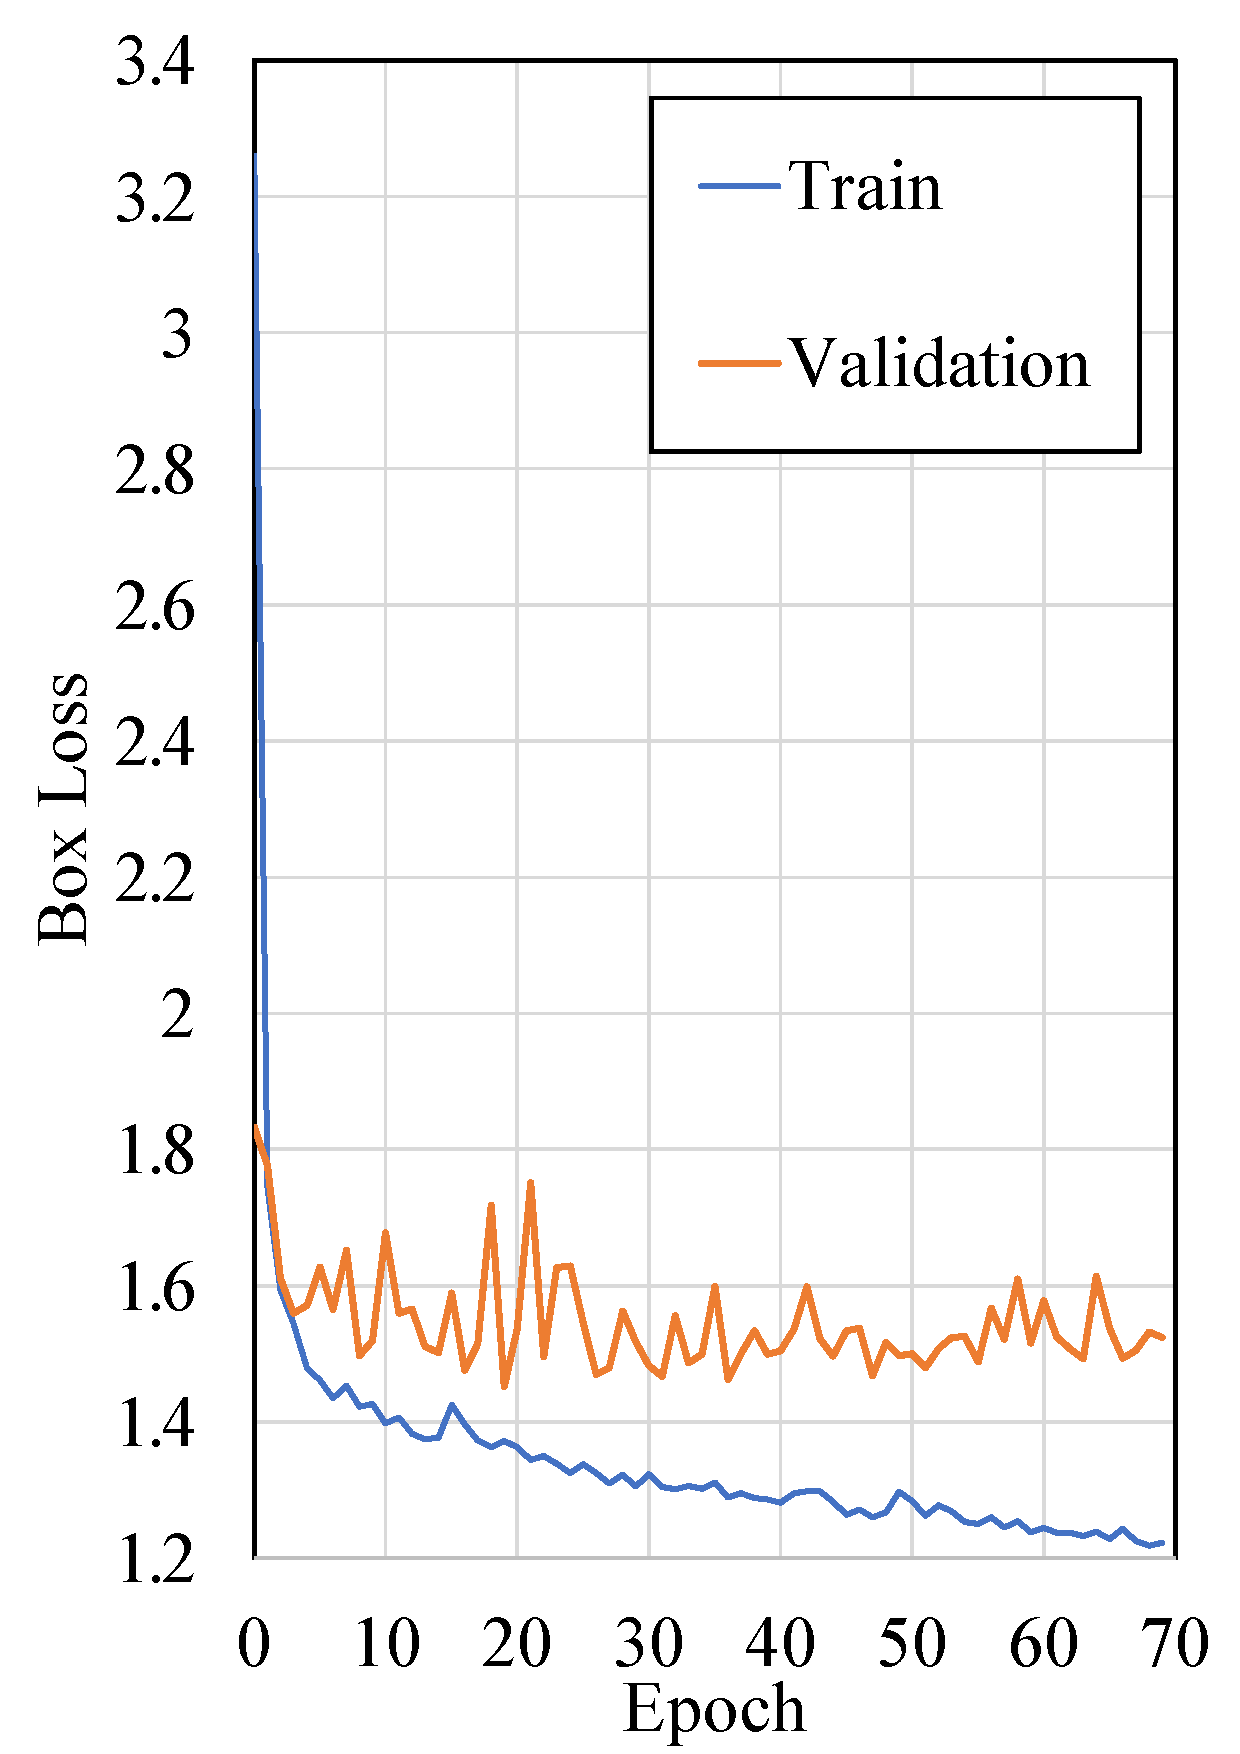
\includegraphics[width=0.333\linewidth]{Images/box2.pdf}\hfill
  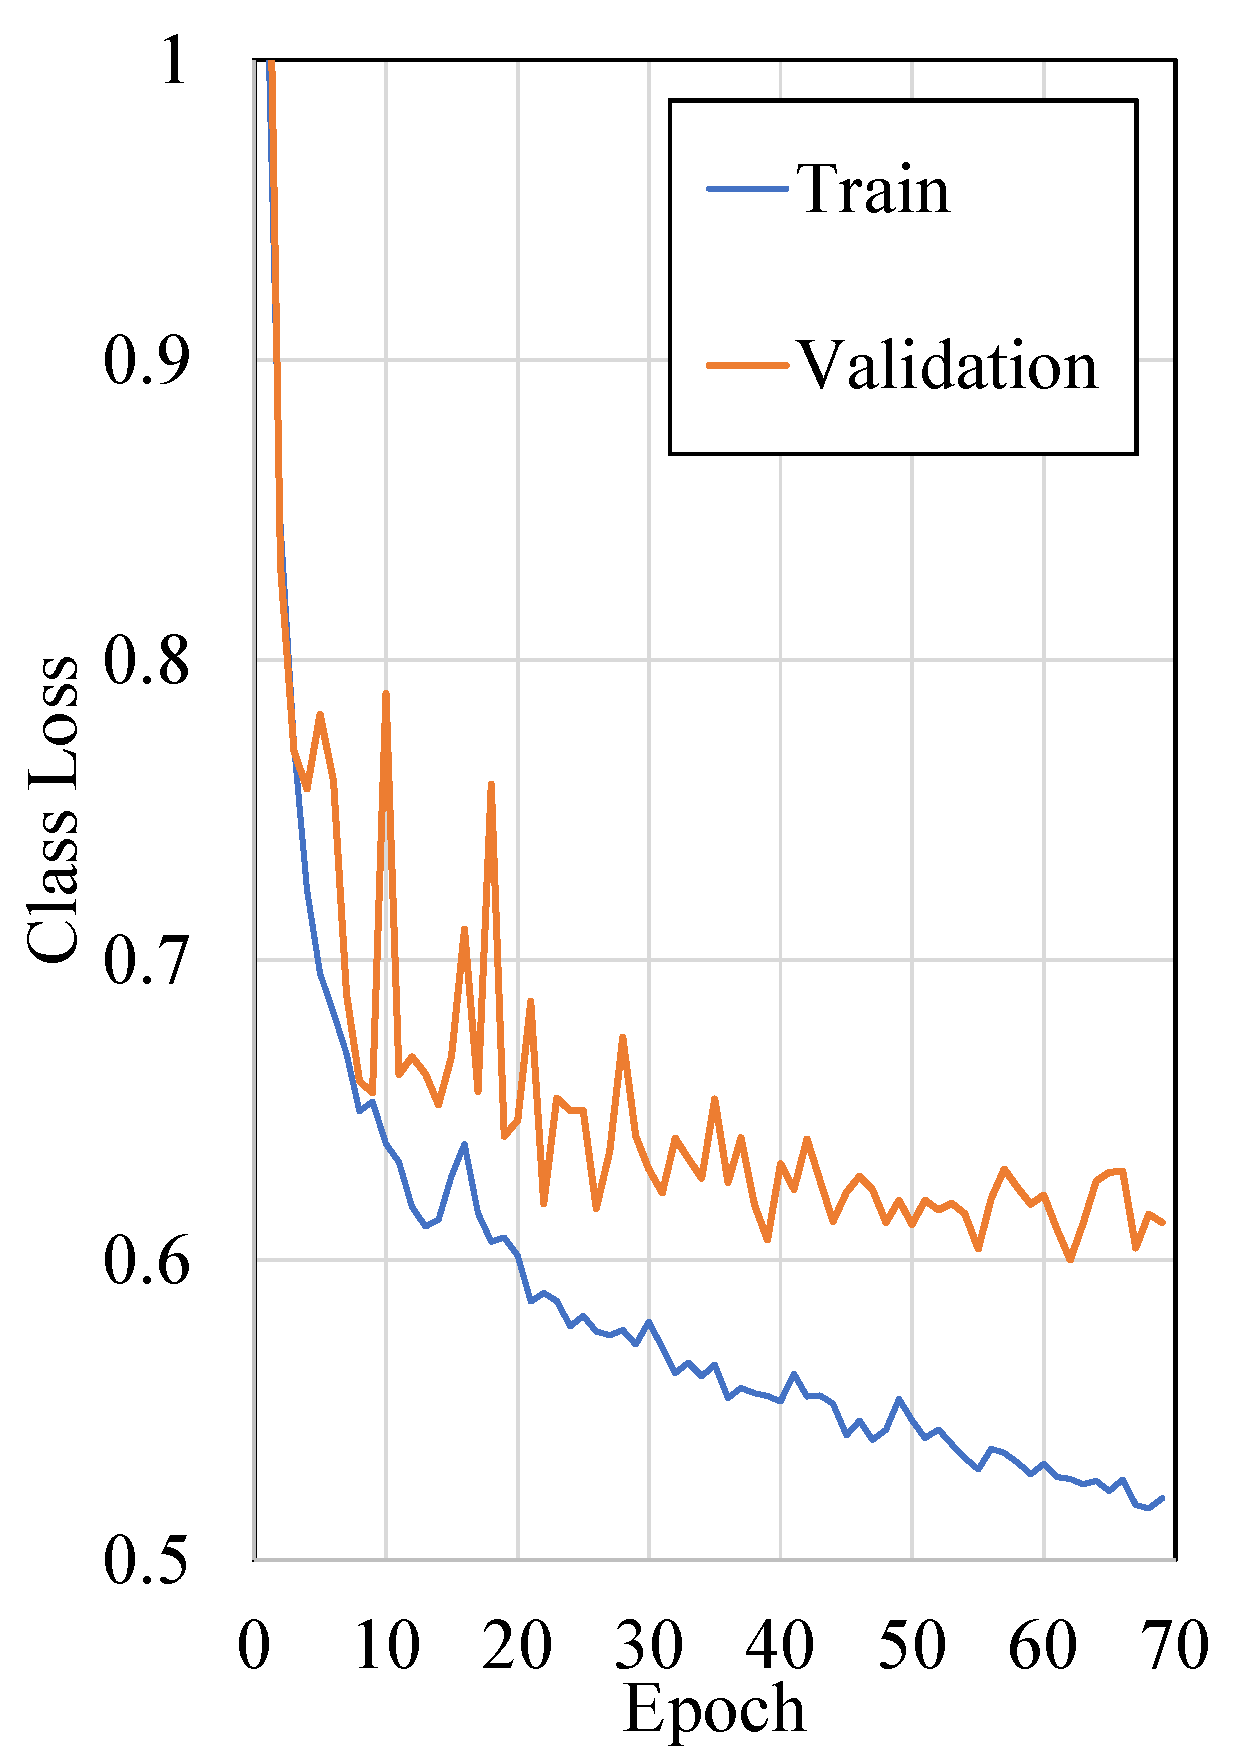
\includegraphics[width=0.333\linewidth]{Images/clss2.pdf}\hfill
  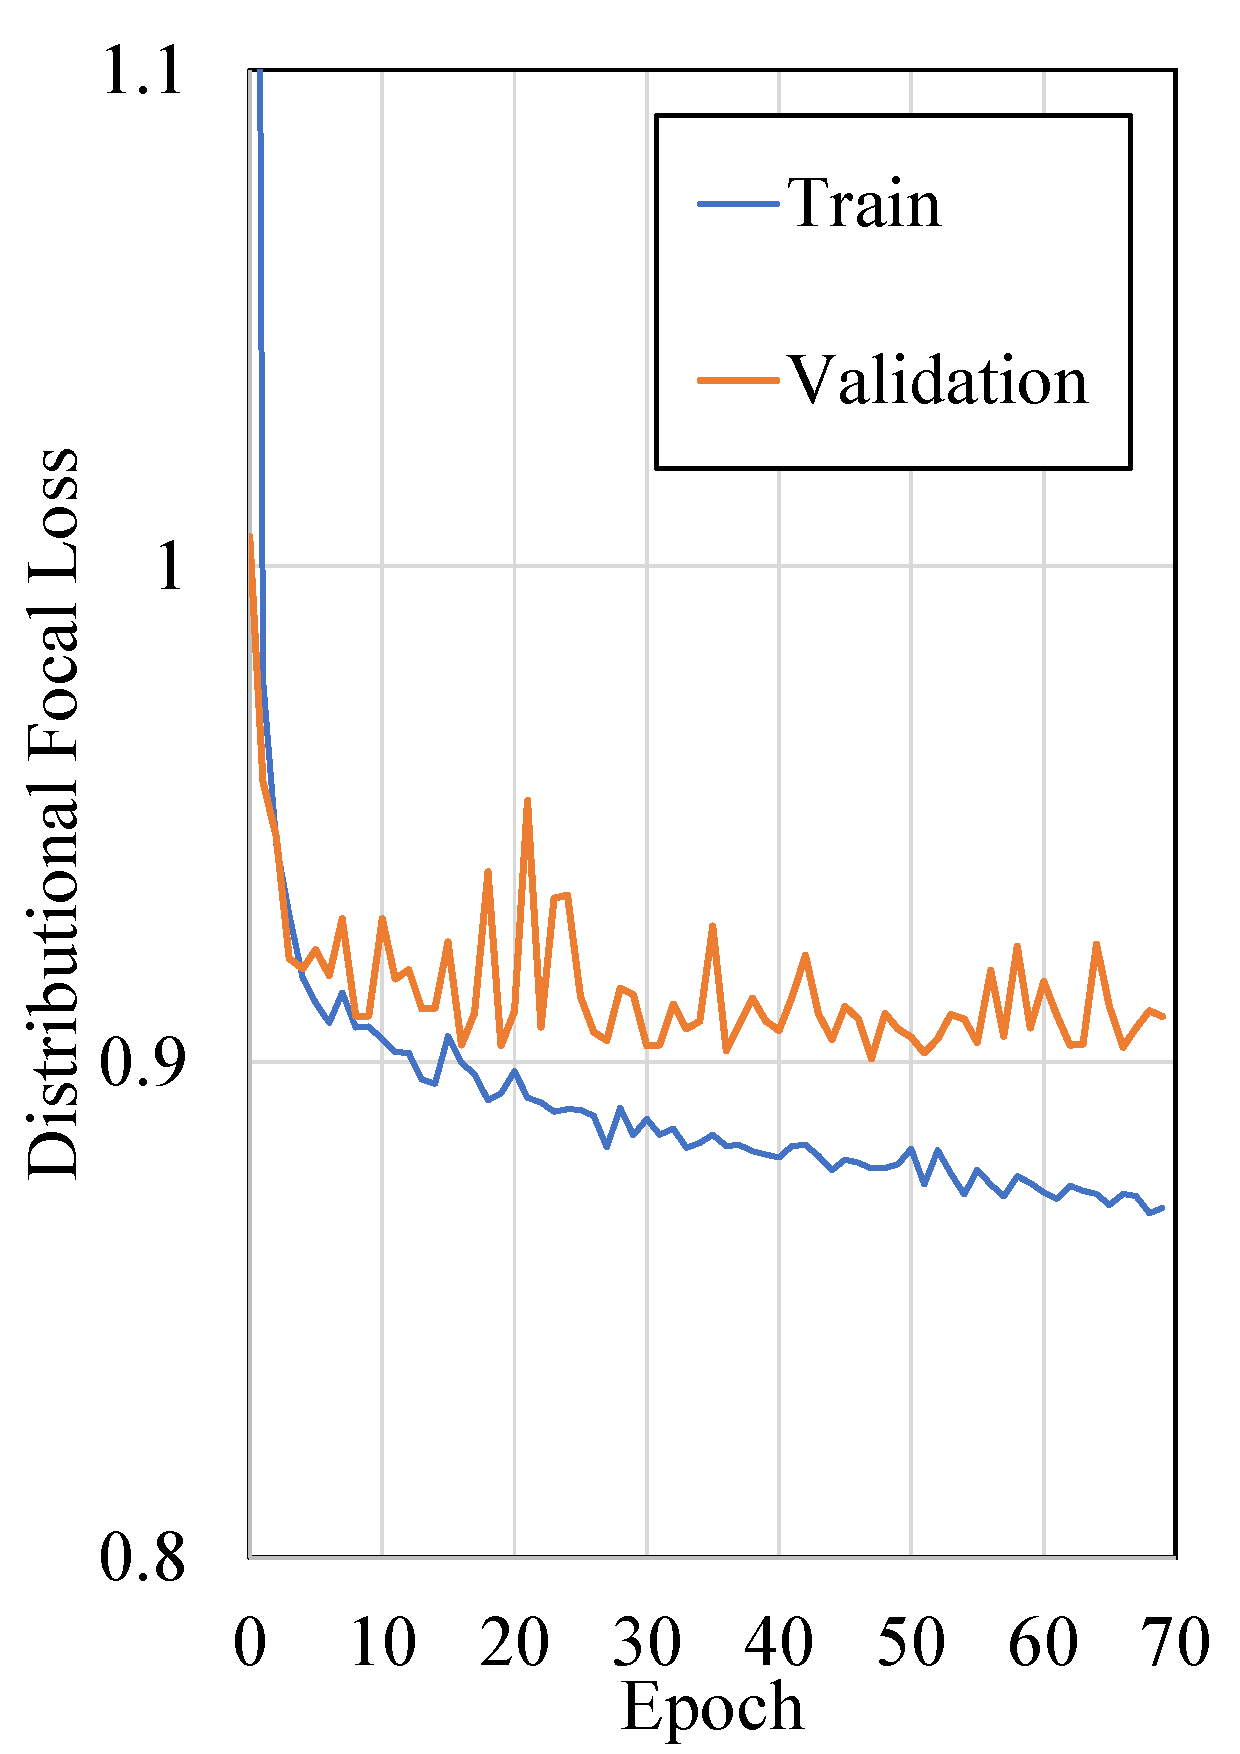
\includegraphics[width=0.333\linewidth]{Images/dfl2.pdf}%
  \end{minipage}%
  \caption{Final Model Train/Validation Comparison}
  \label{final}
\end{figure}

The above figure shows that after a certain number of epochs, the training losses decrease when the training continues. This is from the model overfitting to the training set. If the model continues training after this stage, the accuracy of the model in validation and test sets will degrade. Therefore, although the training was initially planned for 100 epochs, it stopped at 70, and the model at the 50\textsuperscript{th} epoch was extracted to be used. The final results of the model in the train, validation, and test sets are in Table \ref{finaltable}.

\begin{table}[h]
\centering
\begin{tabular}{|cc|cc|cc|}
\hline
\multicolumn{2}{|c|}{\textbf{Train}} & \multicolumn{2}{c|}{\textbf{Validation}} & \multicolumn{2}{c|}{\textbf{Test}} \\ \hline
\multicolumn{1}{|c|}{mAP50} & mAP50-95 & \multicolumn{1}{c|}{mAP50} & mAP50-95 & \multicolumn{1}{c|}{mAP50} & mAP50-95 \\ \hline
\multicolumn{1}{|c|}{97.3\%} & 61.3\% & \multicolumn{1}{c|}{96.8\%} & 54.0\% & \multicolumn{1}{c|}{96.3\%} & 58.7\% \\ \hline
\end{tabular}%
\caption{Final Model Results}
\label{finaltable}
\end{table}

Although the mAP50 of the testing set only increased by 0.3\% from the preliminary training results, the other accuracy metric, mAP 50-95, has increased more than 2\%. That means the overall quality of detection has increased by a margin. 
\newpage
Another way to evaluate the model's performance is by addressing the model's precision and recall. In object detection tasks, precision is how many of the model's detections passed the IOU threshold (i.e., 50\%). Recall means how many ground truths were detected by the model with higher IOUs than the threshold. They are often defined as the following equations:
\begin{equation}
    Precision = \frac{True Positive}{True Positive + False Positive}
    \label{precision}
\end{equation}
\begin{equation}
    Recall = \frac{True Positive}{True Positive + False Nagative}
\end{equation}

In ideal cases, with no false positives or negatives, both numbers become 1. But in real cases, they are often in a trade-off relationship. If the confidence threshold is lowered, the number of false positives will increase, lowering the precision of the model. In contrast, the number of false negatives will decrease, increasing the recall of the model. Because of this relationship, most precision-recall curves form a downward slope. The more reaching the top right corner, the better. Figure \ref{prcurve} shows the precision-recall curve of this model.

\begin{figure}[h]
    \centering
    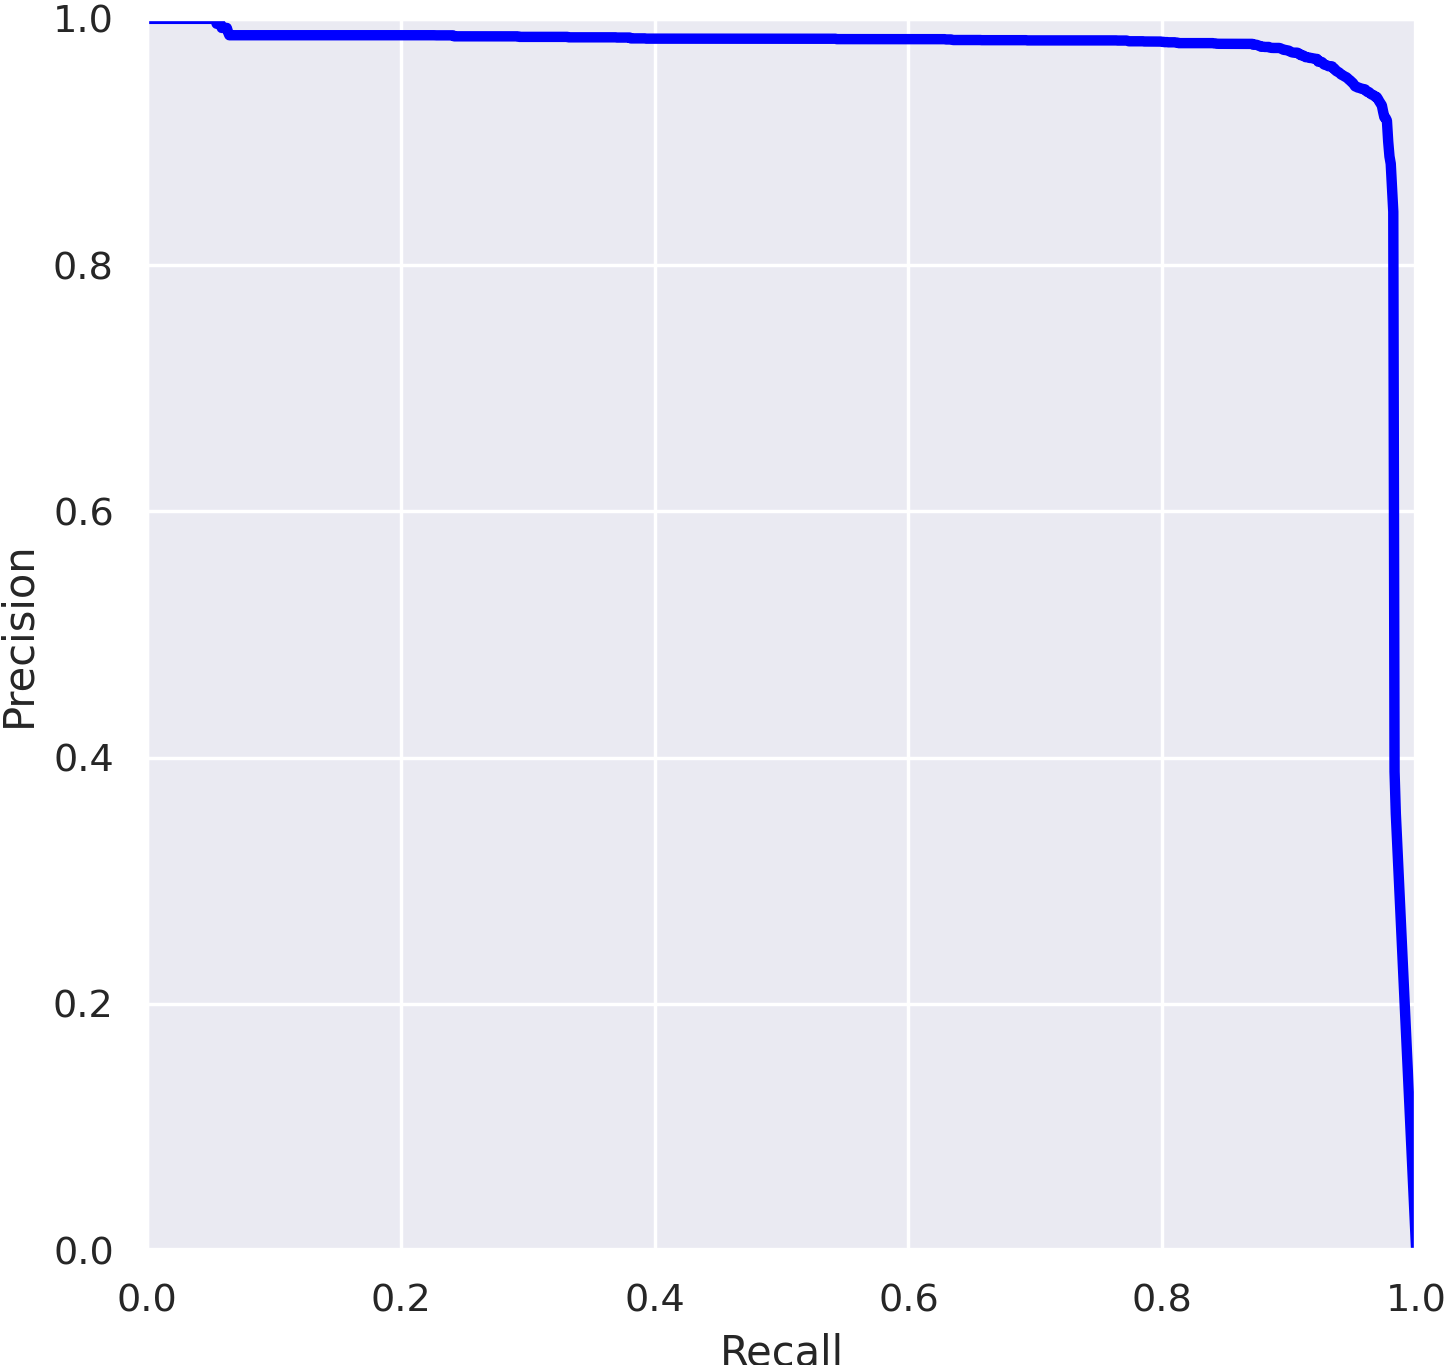
\includegraphics[width=0.7\textwidth]{Images/PR_curve.png}
    \caption{Precision-Recall Curve}
    \label{prcurve}
\end{figure}

Figure \ref{prcurve} shows that this model is robust against false positives and negatives. The model maintains more than 93\% precision and recall through the whole confidence threshold range. Moreover, an F1 score can be calculated to find the optimal confidence threshold for the highest precision and recall simultaneously. The calculation method of the F1 score is as follows.

\begin{equation}
    F1 Score = \frac{2 \times (Precision \times Recall)}{Precision+Recall}
    \label{f1score}
\end{equation}

Then, a graph can be plotted for F1 scores against different confidence values. 

\begin{figure}[h]
    \centering
    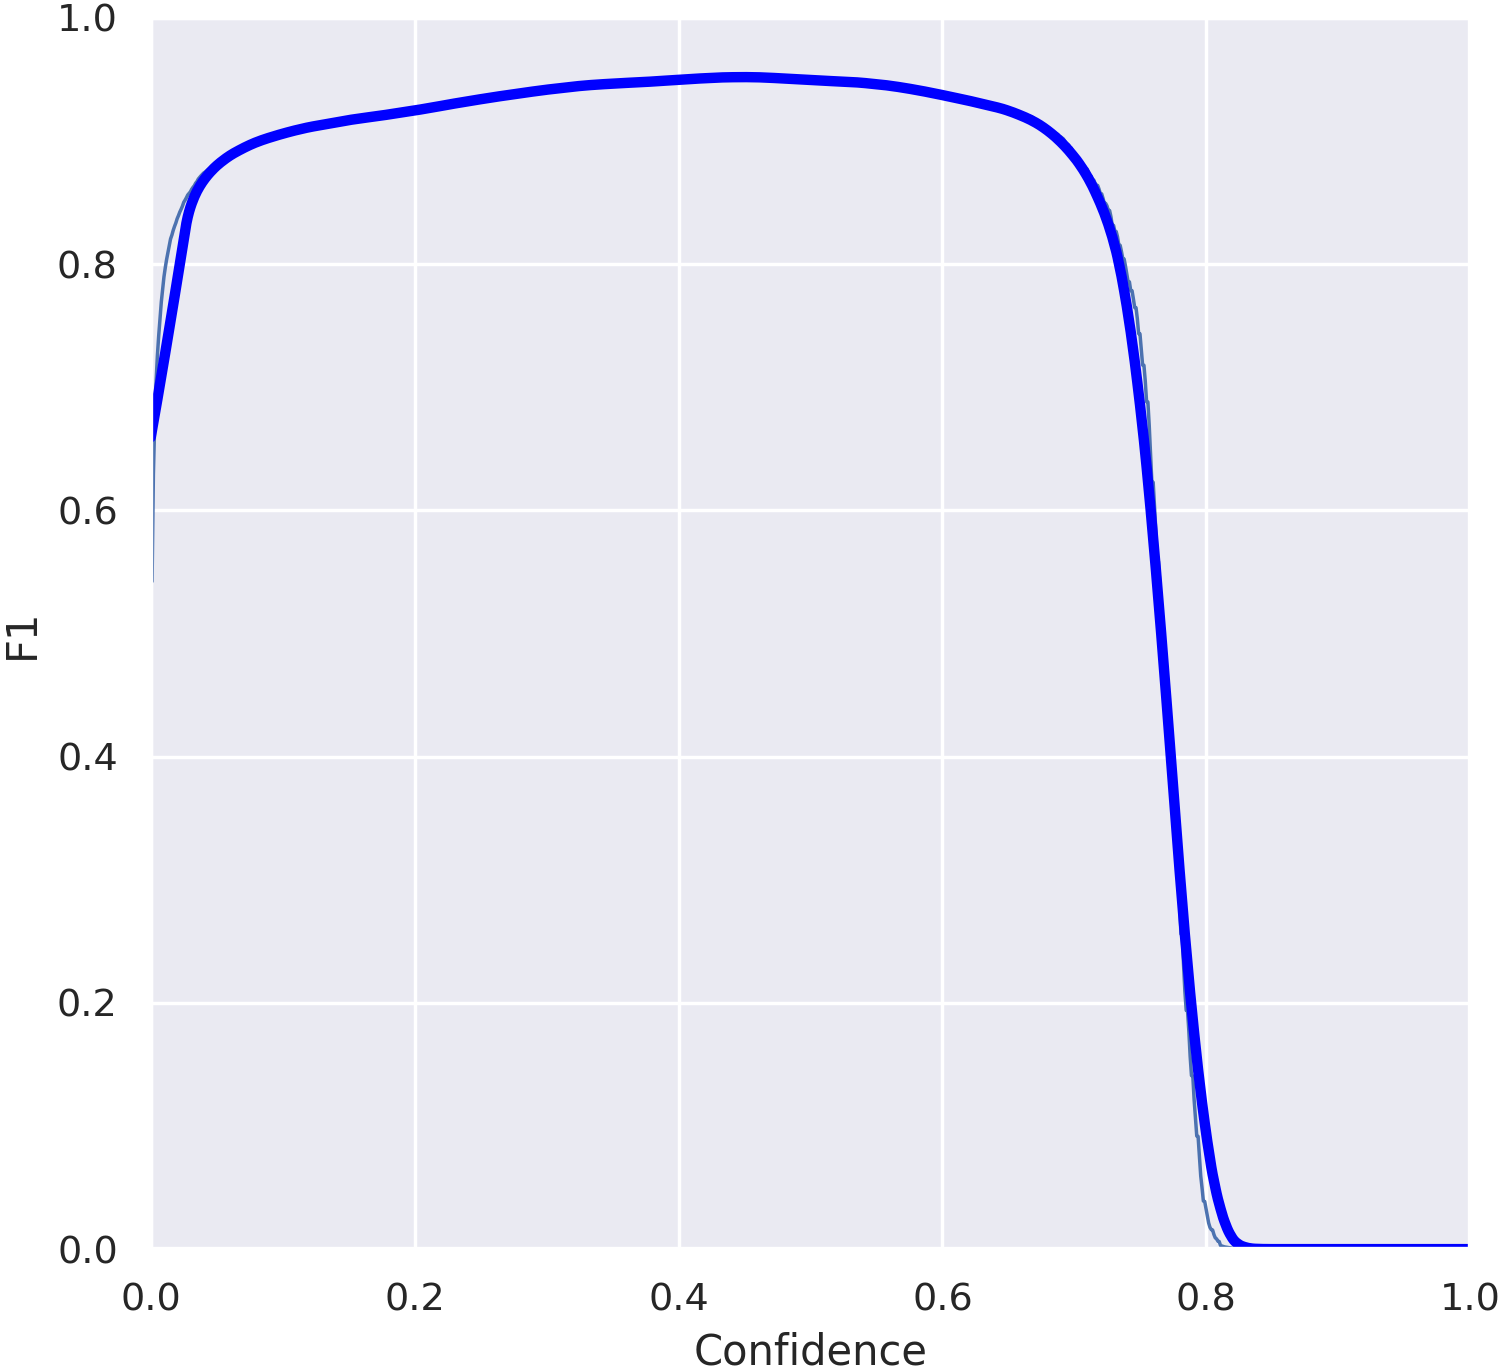
\includegraphics[width=0.7\textwidth]{Images/F1_curve.png}
    \caption{F1-Confidence Curve}
    \label{f1curve}
\end{figure}

Figure \ref{f1curve} shows the optimal confidence value of 0.45. This value will be used for the model during the tracking process.

The following figures are the prediction results from the model in the validation and test sets. Along with the detection, there are the class name and the confidence score. 

\begin{figure}
    \centering
    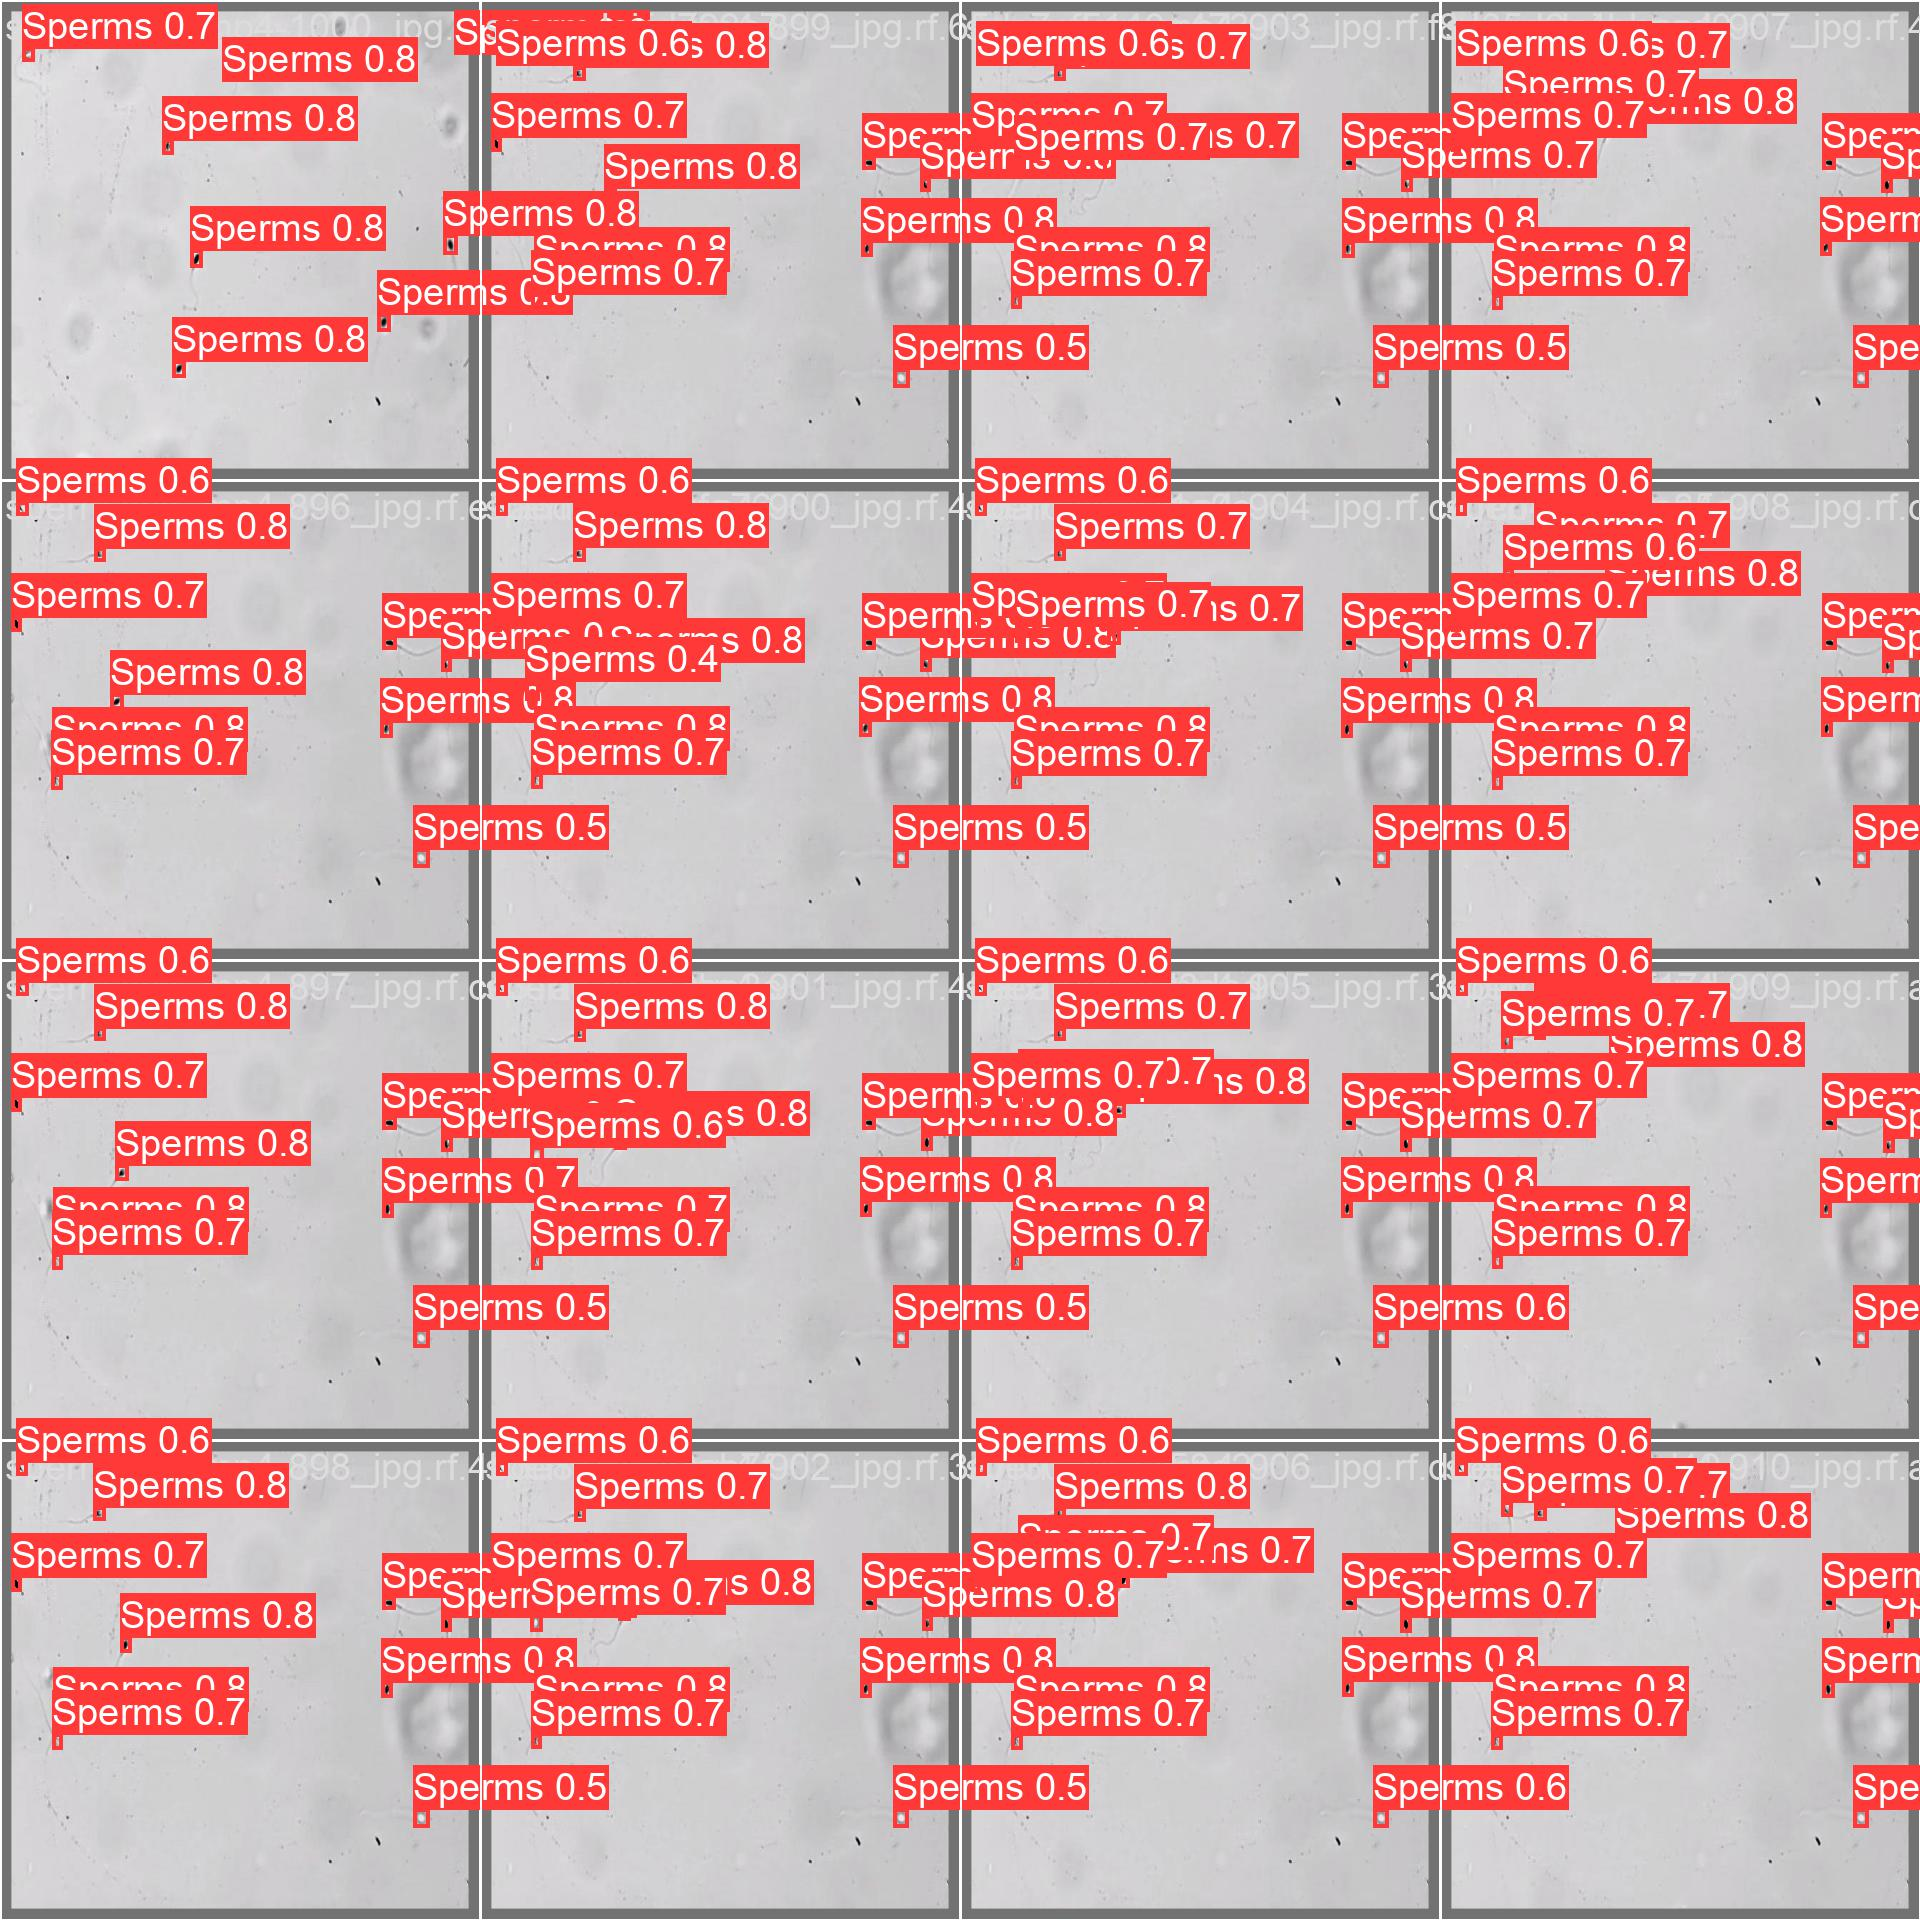
\includegraphics[width=\textwidth]{Images/val_batch0_pred.jpg}
    \caption{Validation Set Prediction}
    \label{valpred}
\end{figure}

\begin{figure}
    \centering
    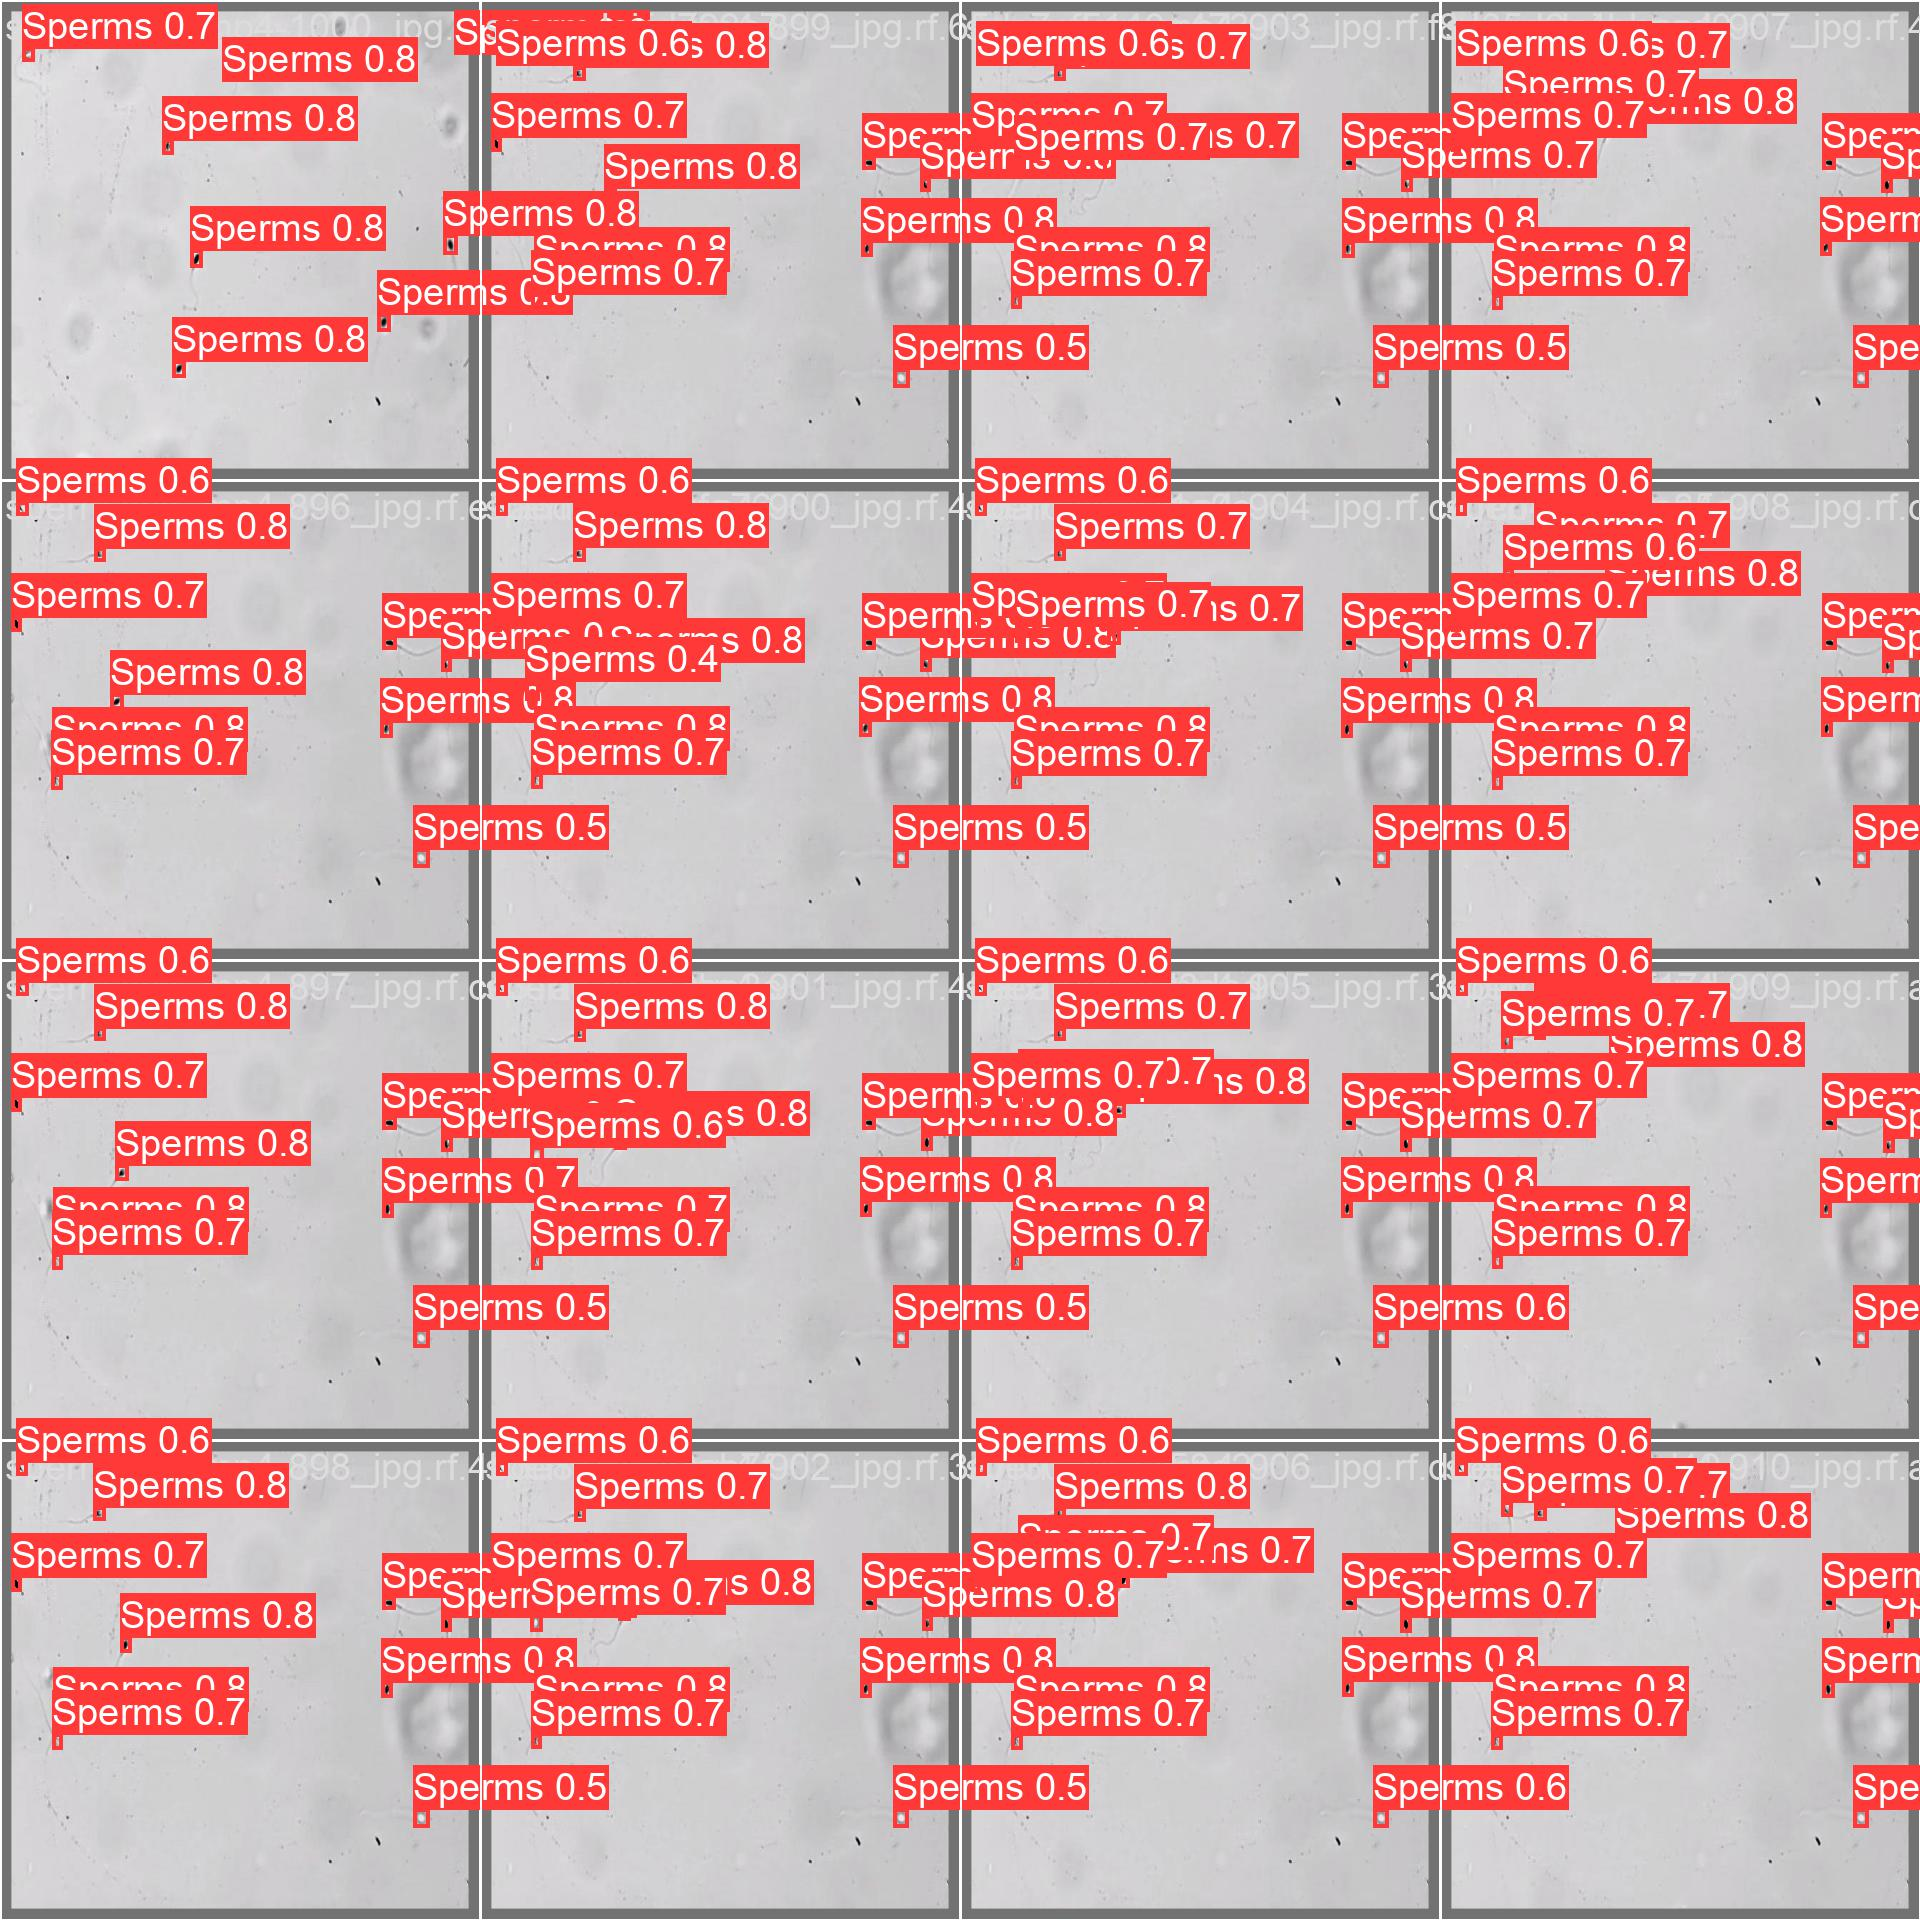
\includegraphics[width=\textwidth]{Images/val_batch0_pred (1).jpg}
    \caption{Test Set Prediction}
    \label{testpred}
\end{figure}
\newpage
\section{Tracking Result}
Five video samples with different characteristics were extracted to test this program's tracking function. The first three samples had high, medium, and low counts of sperms. These three samples will evaluate the performance of the tracking program in situations with different probabilities of occlusion, as more sperms will lead to more crossing-overs between them. Moreover, this will test the program's ability to handle real-time tracking since more calculations will be needed for more sperms. Figure \ref{sam1-3} shows the snapshot of each sample. 

\begin{figure}[h]
     \centering
     \begin{subfigure}[b]{0.31\textwidth}
         \centering
         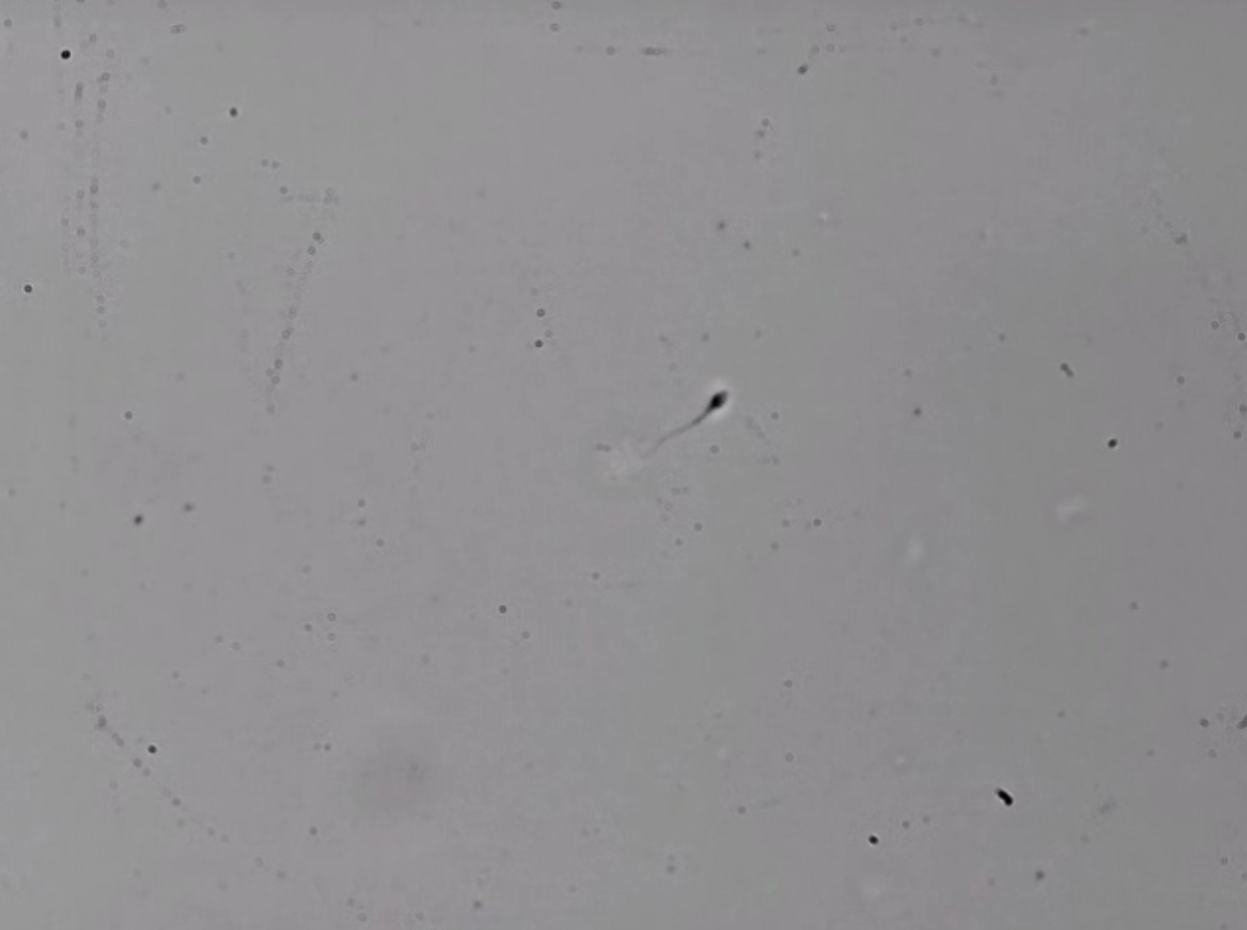
\includegraphics[width=\textwidth]{Images/low.png}
         \caption{Sample 1: Low}
         \label{sam1}
     \end{subfigure}
     \hfill
     \begin{subfigure}[b]{0.31\textwidth}
         \centering
         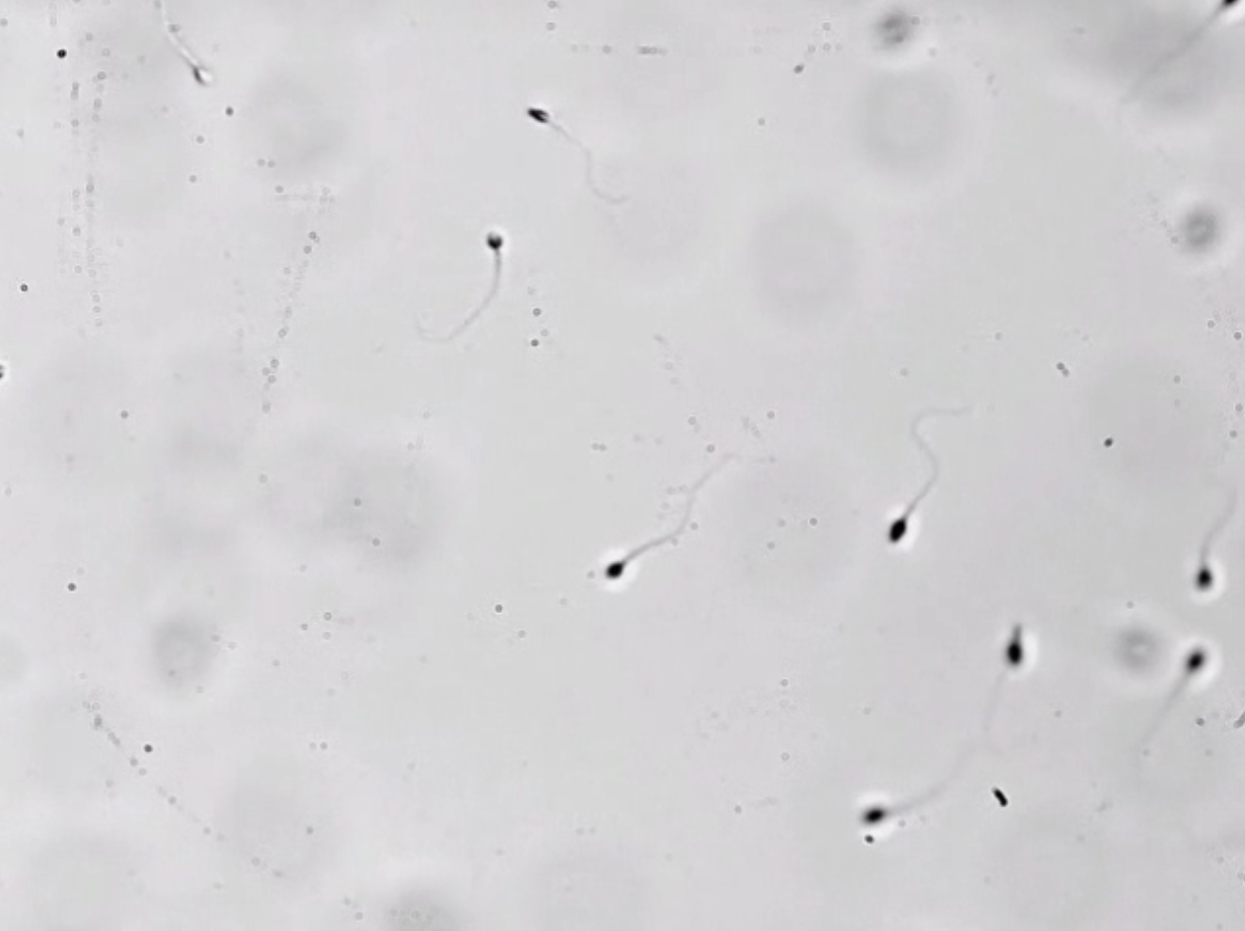
\includegraphics[width=\textwidth]{Images/med.png}
         \caption{Sample 2: Medium}
         \label{sam2}
     \end{subfigure}
     \hfill
     \begin{subfigure}[b]{0.31\textwidth}
         \centering
         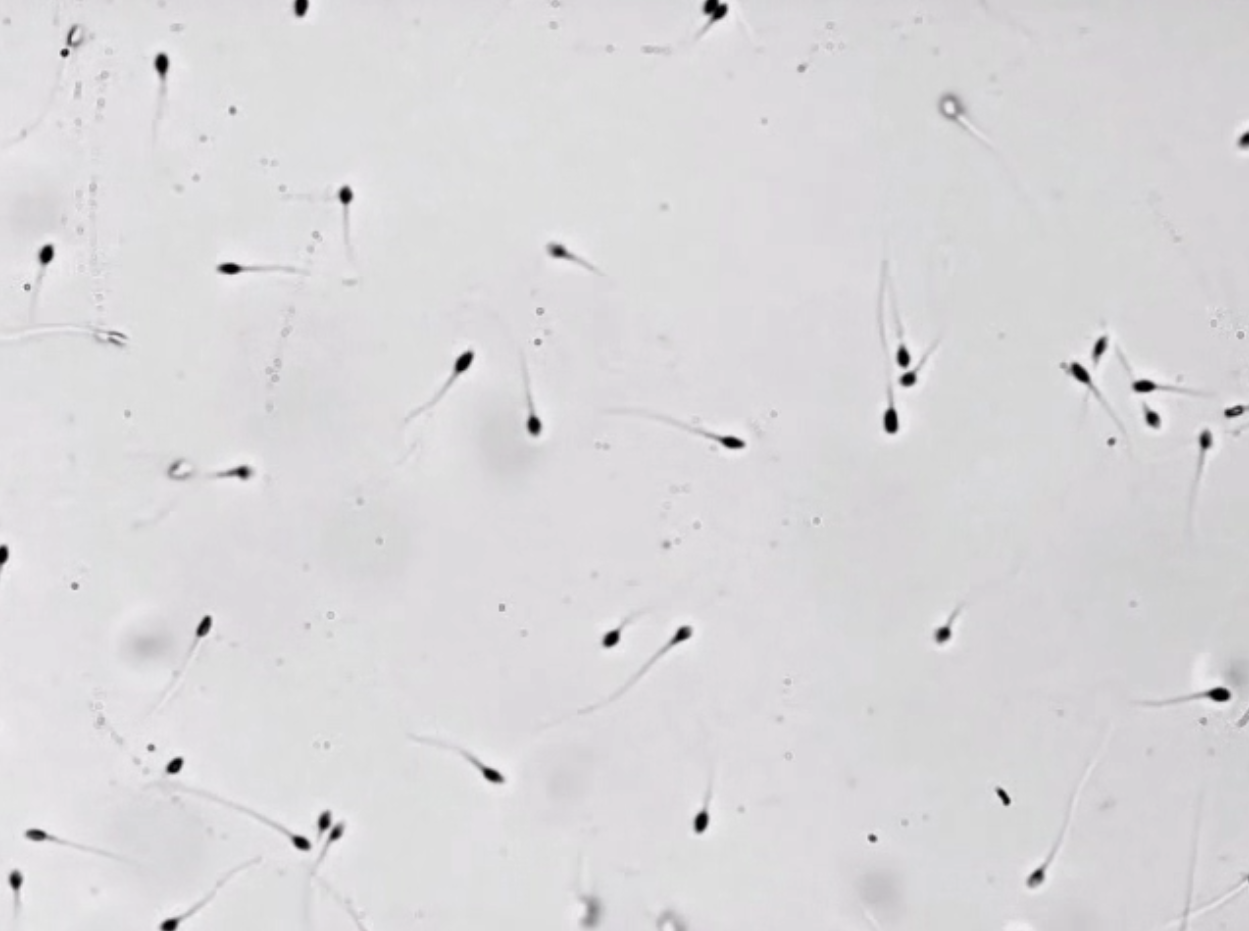
\includegraphics[width=\textwidth]{Images/high.png}
         \caption{Sample 3: High}
         \label{sam3}
     \end{subfigure}
        \caption{Tracking Samples 1-3}
        \label{sam1-3}
\end{figure}

The remaining two samples will test the program's robustness to blurry sperms. The program will be particularly examined for its ability to detect and track blurry sperms and its capacity to predict the tracks of blurry sperms when it is undetected by the model for multiple frames. Figure \ref{sam4-5} shows the snapshot of the last two testing samples.

\begin{figure}[h]
     \centering
     \begin{subfigure}[b]{0.46\textwidth}
         \centering
         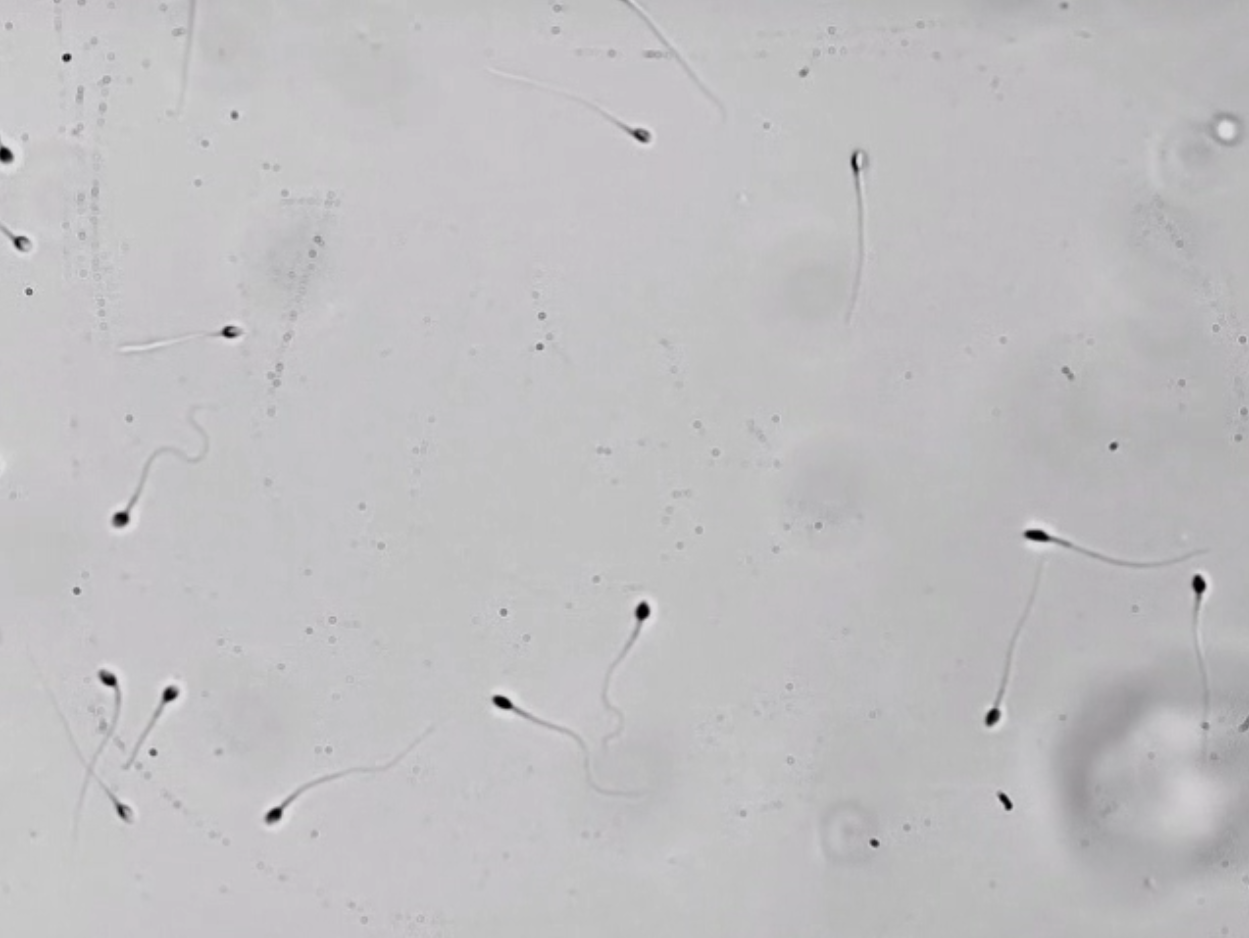
\includegraphics[width=\textwidth]{Images/clear.png}
         \caption{Sample 4: Clear}
         \label{sam4}
     \end{subfigure}
     \hfill
     \begin{subfigure}[b]{0.46\textwidth}
         \centering
         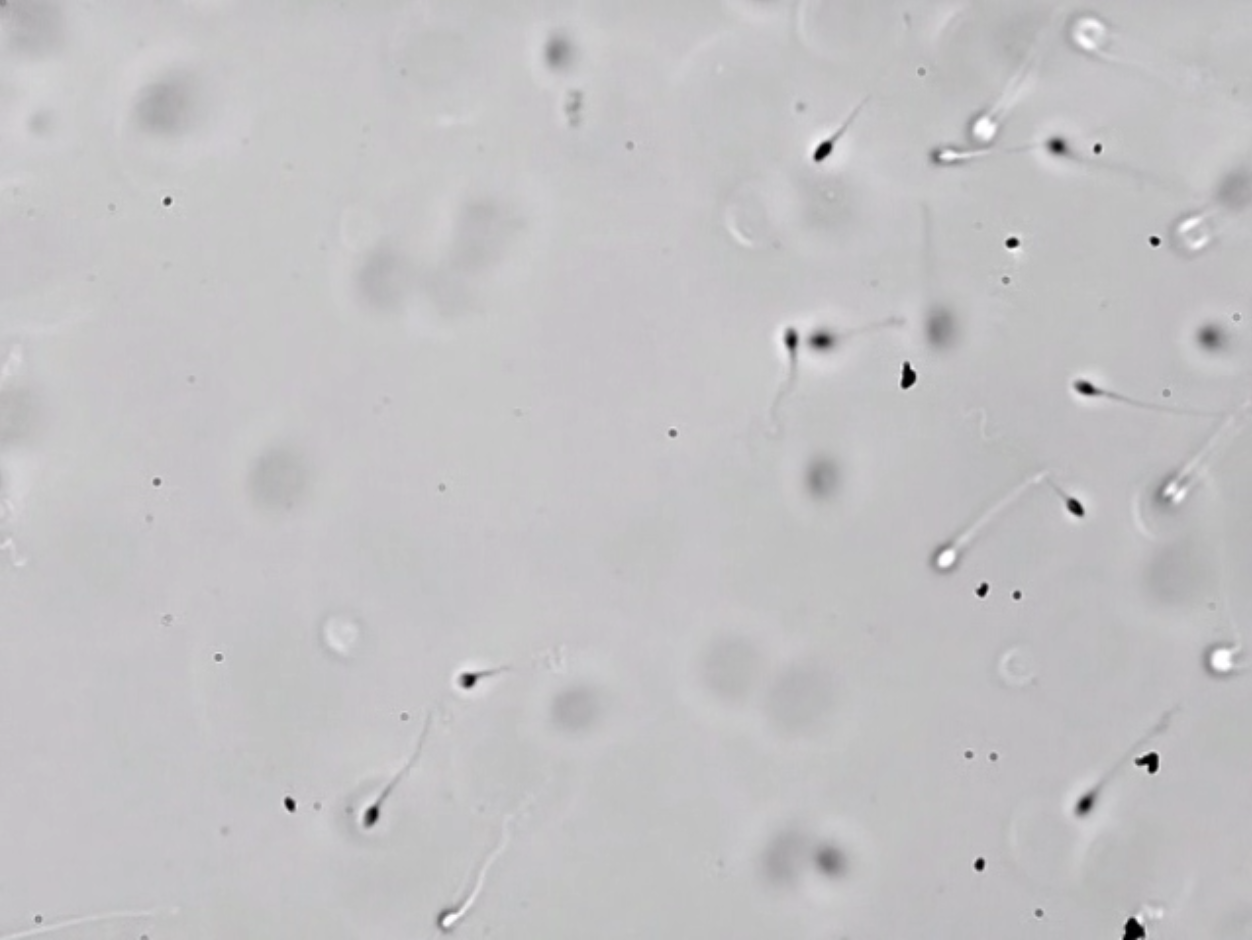
\includegraphics[width=\textwidth]{Images/blurry.png}
         \caption{Sample 5: Blurry}
         \label{sam5}
     \end{subfigure}
        \caption{Tracking Samples 4-5}
        \label{sam4-5}
\end{figure}
The sample videos and the program output videos are available at \href{https://github.com/rladntjr7/FYP}{\underline{GitHub}}.


As shown in Figure \ref{sam4-5}, Sample 4 has the sperms that clearly indicate the sperm heads. Whereas Sample 5 contains many sperms that appear not as clearly as those from Sample 4. It can be speculated that those sperms that are not perfectly focused from the camera appear white and round. As shown in Figure \ref{valpred} and  Figure \ref{testpred}, these kinds of sperms tend to have lower confidence scores than those with more clear shapes. This will lead to those sperms intermittently detected by the model, testing the occlusion tracking function. 

\subsubsection{Sample 1: Low Count}
Figure \ref{sam1res} shows the snapshot of the program output of sample 1. 
\begin{figure}[h]
    \centering
    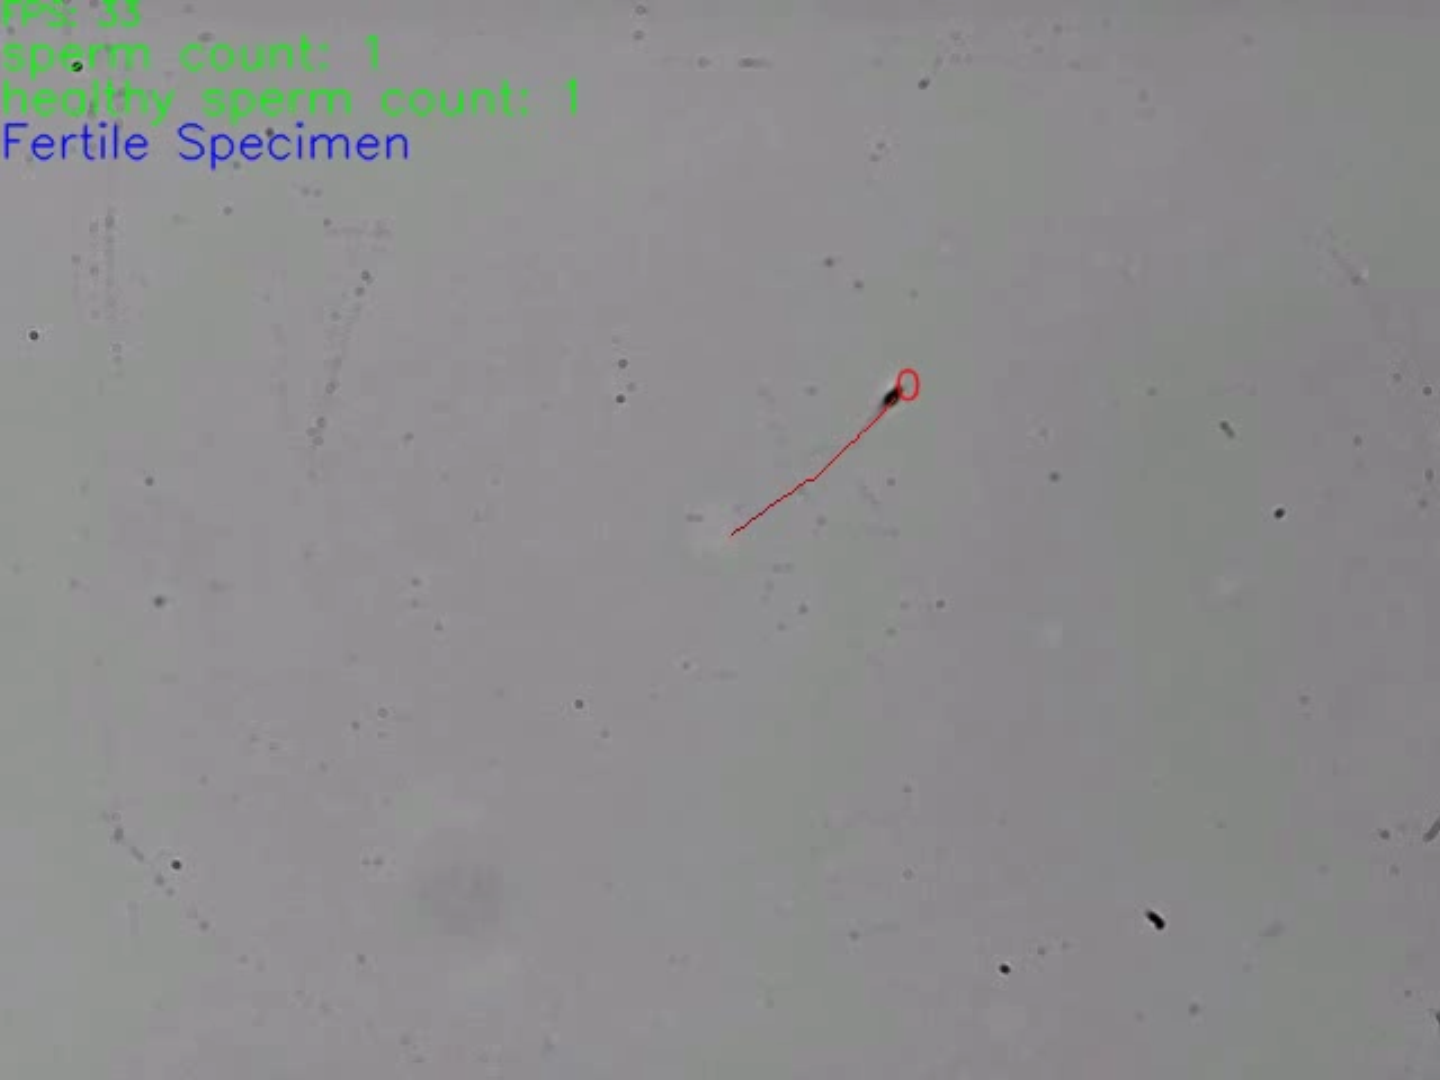
\includegraphics[width=0.75\textwidth]{Images/sam1.png}
    \caption{Sample 1 Output}
    \label{sam1res}
\end{figure}

With one sperm, the model had a satisfactory result. The FPS was over 30 throughout the video, and the ID number correctly followed the sperm head without any ID switch. 

\newpage
\subsubsection{Sample 2: Medium Count}
Figure \ref{sam2res} shows the snapshot of the program output of sample 2.
\begin{figure}[h]
    \centering
    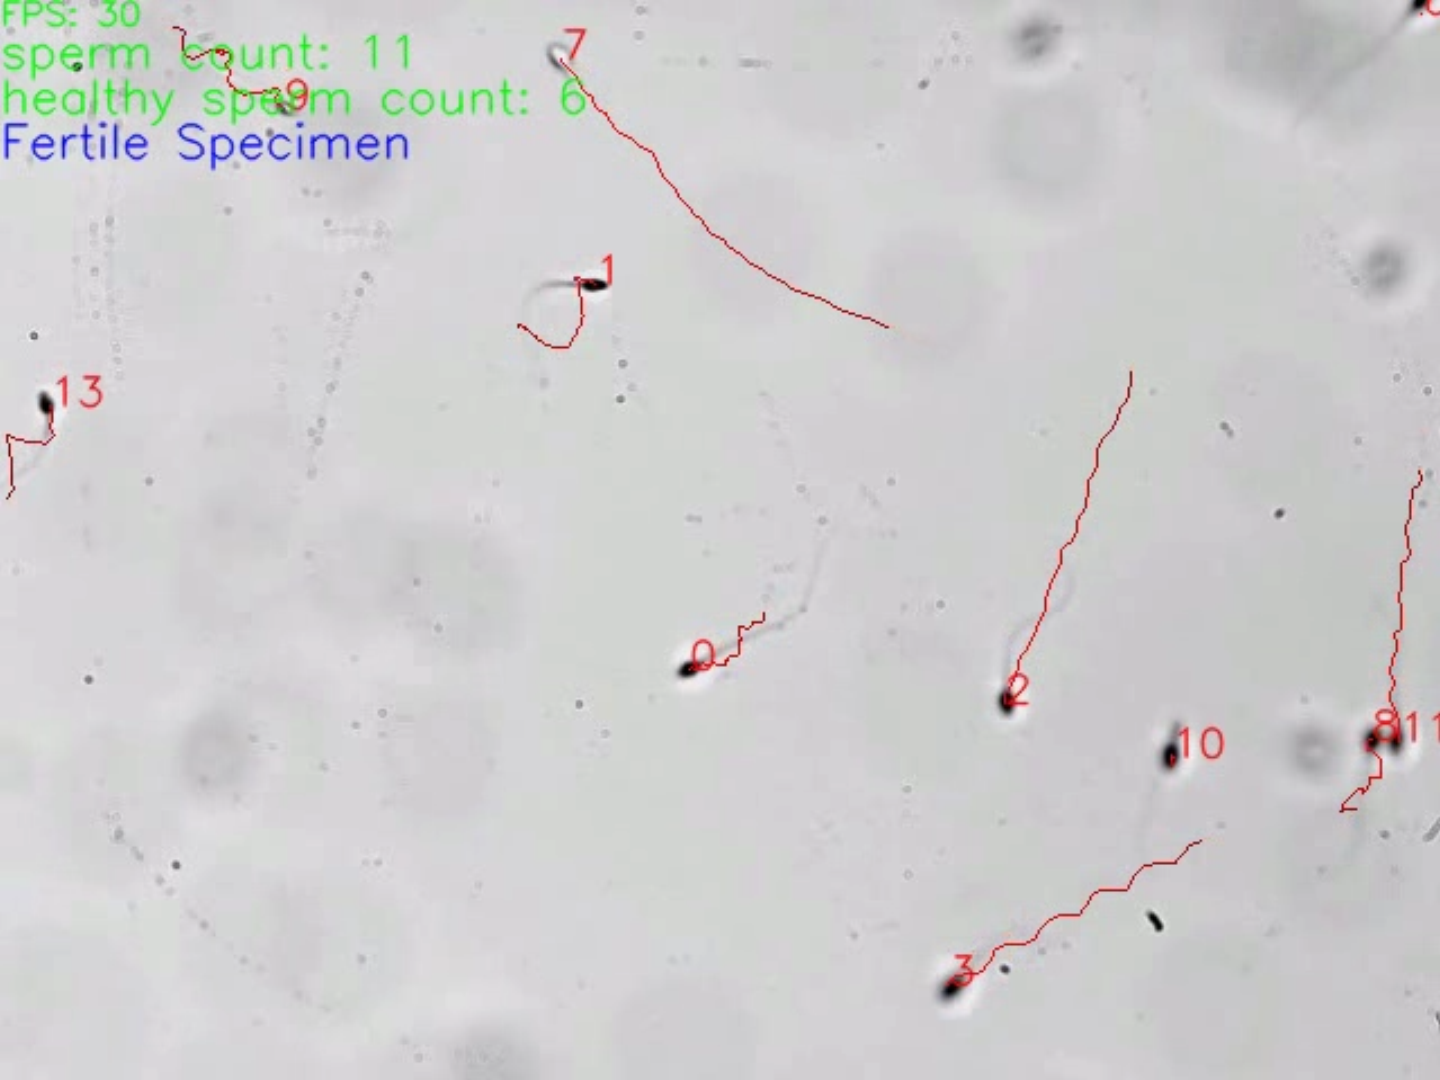
\includegraphics[width=0.75\textwidth]{Images/sam2.png}
    \caption{Sample 2 Output}
    \label{sam2res}
\end{figure}

With multiple sperms in one frame, the program also had a satisfactory result, maintaining 30 frames per second. On the right of Figure \ref{sam2res}, sperm 8 and 11 were moving very closely with each other, but there was no ID switch between them. Moreover, the program deals well with the complex trajectory of sperm 1 and 13, as shown in Figure \ref{sam22}.
\begin{figure}[h]
     \centering
     \begin{subfigure}[b]{0.35\textwidth}
         \centering
         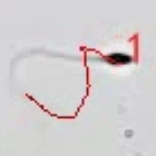
\includegraphics[width=\textwidth]{Images/sam222.png}
     \end{subfigure}
     \hspace{4em}%
     \begin{subfigure}[b]{0.35\textwidth}
         \centering
         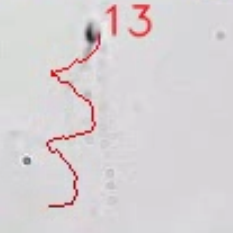
\includegraphics[width=\textwidth]{Images/sam22.png}
     \end{subfigure}
        \caption{Trajectories of Sperm 1 and 13 in Sample 2}
        \label{sam22}
\end{figure}
\newpage
\subsubsection{Sample 3: High Count}
Figure \ref{sam3res} shows the snapshot of the program output of sample 3.
\begin{figure}[h]
    \centering
    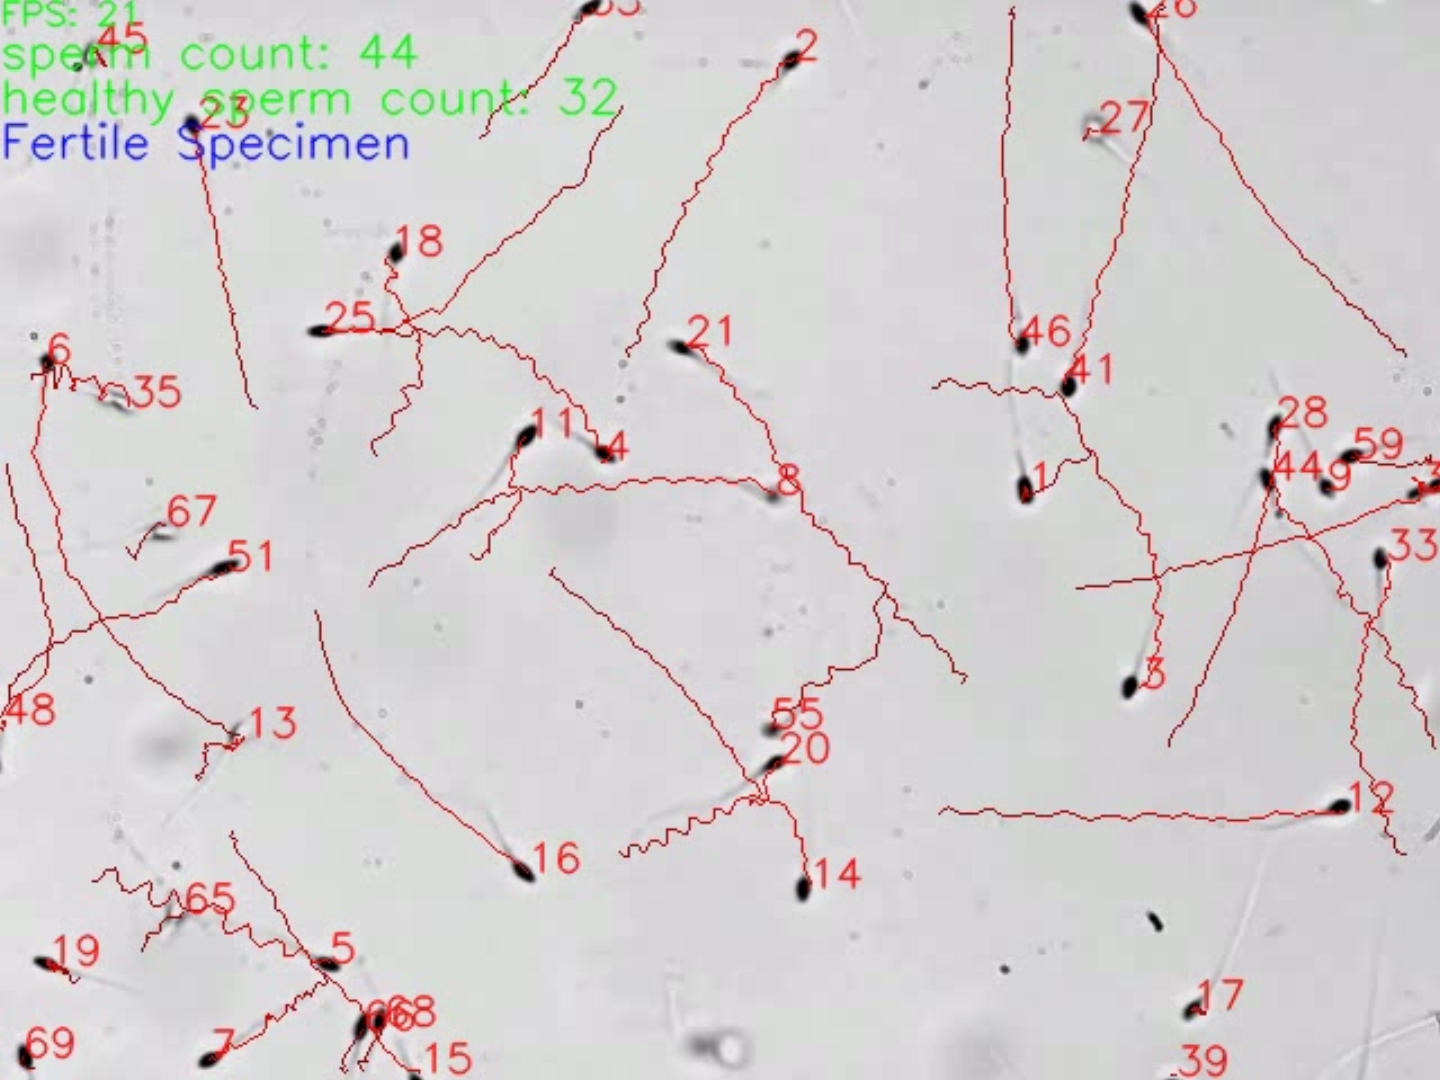
\includegraphics[width=0.75\textwidth]{Images/sam3.png}
    \caption{Sample 3 Output}
    \label{sam3res}
\end{figure}

With many sperms in one frame, the FPS slowed significantly to 20. Also, many collisions and cross-overs were taking place. The model handled some very well, as shown in Figure \ref{sam3col}.
\begin{figure}[h]
     \centering
     \begin{subfigure}[b]{0.34\textwidth}
         \centering
         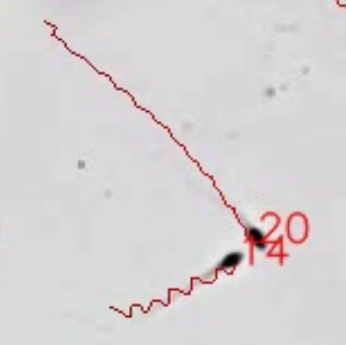
\includegraphics[width=\textwidth]{Images/sam33.png}
     \end{subfigure}
     \hspace{4em}%
     \begin{subfigure}[b]{0.34\textwidth}
         \centering
         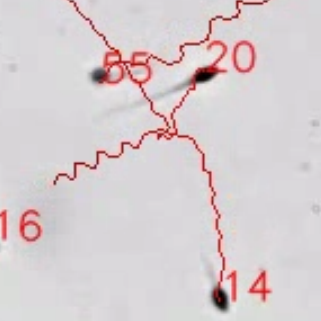
\includegraphics[width=\textwidth]{Images/sam333.png}
     \end{subfigure}
        \caption{Cross-Over of Sperm 14 and 20 in Sample 3}
        \label{sam3col}
\end{figure}

Sperms 14 and 20 had a cross-over, but the program calculated the most probable trajectories of each sperm, and no ID switching occurred.
\newpage
Although not many, ID switching was still occurring due to the rapid movement and collisions of sperms. 

\begin{figure}[ht]
     \centering
     \begin{subfigure}[b]{0.3\textwidth}
         \centering
         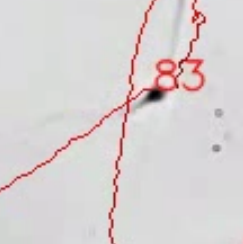
\includegraphics[width=\textwidth]{Images/sam3333.png}
     \end{subfigure}
     \hfill
     \begin{subfigure}[b]{0.3\textwidth}
         \centering
         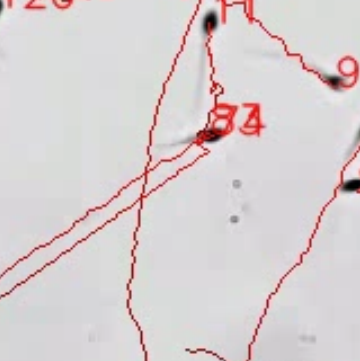
\includegraphics[width=\textwidth]{Images/sam33333.png}
     \end{subfigure}
     \hfill
     \begin{subfigure}[b]{0.3\textwidth}
         \centering
         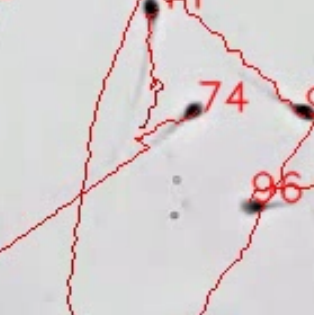
\includegraphics[width=\textwidth]{Images/sam333333.png}
     \end{subfigure}
        \caption{ID Switching of Sperm 83 to 74 in Sample 3}
        \label{sam3sw}
\end{figure}

In Figure \ref{sam3sw}, Sperm 83 was switched to 74. The cause of this switching is track 74 not being permanently disabled after it becomes inactive. Then, the detection at a certain frame was closer to track 74 than its original track, and it switched the ID.

\begin{figure}[h]
     \centering
     \begin{subfigure}[b]{0.3\textwidth}
         \centering
         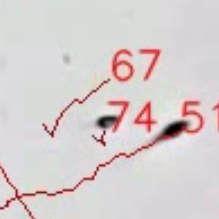
\includegraphics[width=\textwidth]{Images/sam3333333.png}
         \caption{67 \textrightarrow 74}
     \end{subfigure}
     \hfill
     \begin{subfigure}[b]{0.3\textwidth}
         \centering
         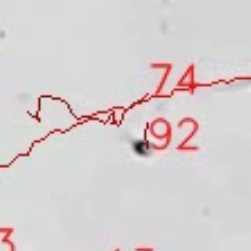
\includegraphics[width=\textwidth]{Images/sam33333333.png}
         \caption{74 \textrightarrow 92}
     \end{subfigure}
     \hfill
     \begin{subfigure}[b]{0.3\textwidth}
         \centering
         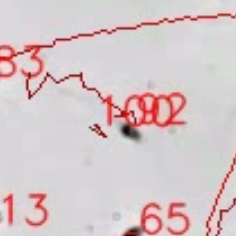
\includegraphics[width=\textwidth]{Images/sam333333333.png}
         \caption{92 \textrightarrow 100}
     \end{subfigure}
        \caption{Sperm with Multiple IDs Assigned in Sample 3}
        \label{sam3mult}
\end{figure}

Figure \ref{sam3mult} shows a sperm assigned to multiple IDs. The sperm's original ID was 56, but whenever it made a sharp turn, the program could not follow the correct trajectory and assigned a new ID. 

These issues do not degrade the model's overall performance significantly because most of the sperms are working well. Still, it can be improved for the quality of the program.

\newpage
\subsubsection{Sample 4: Clear Sperms}
Figure \ref{sam4res} shows the snapshot of the program output of sample 4.
\begin{figure}[h]
    \centering
    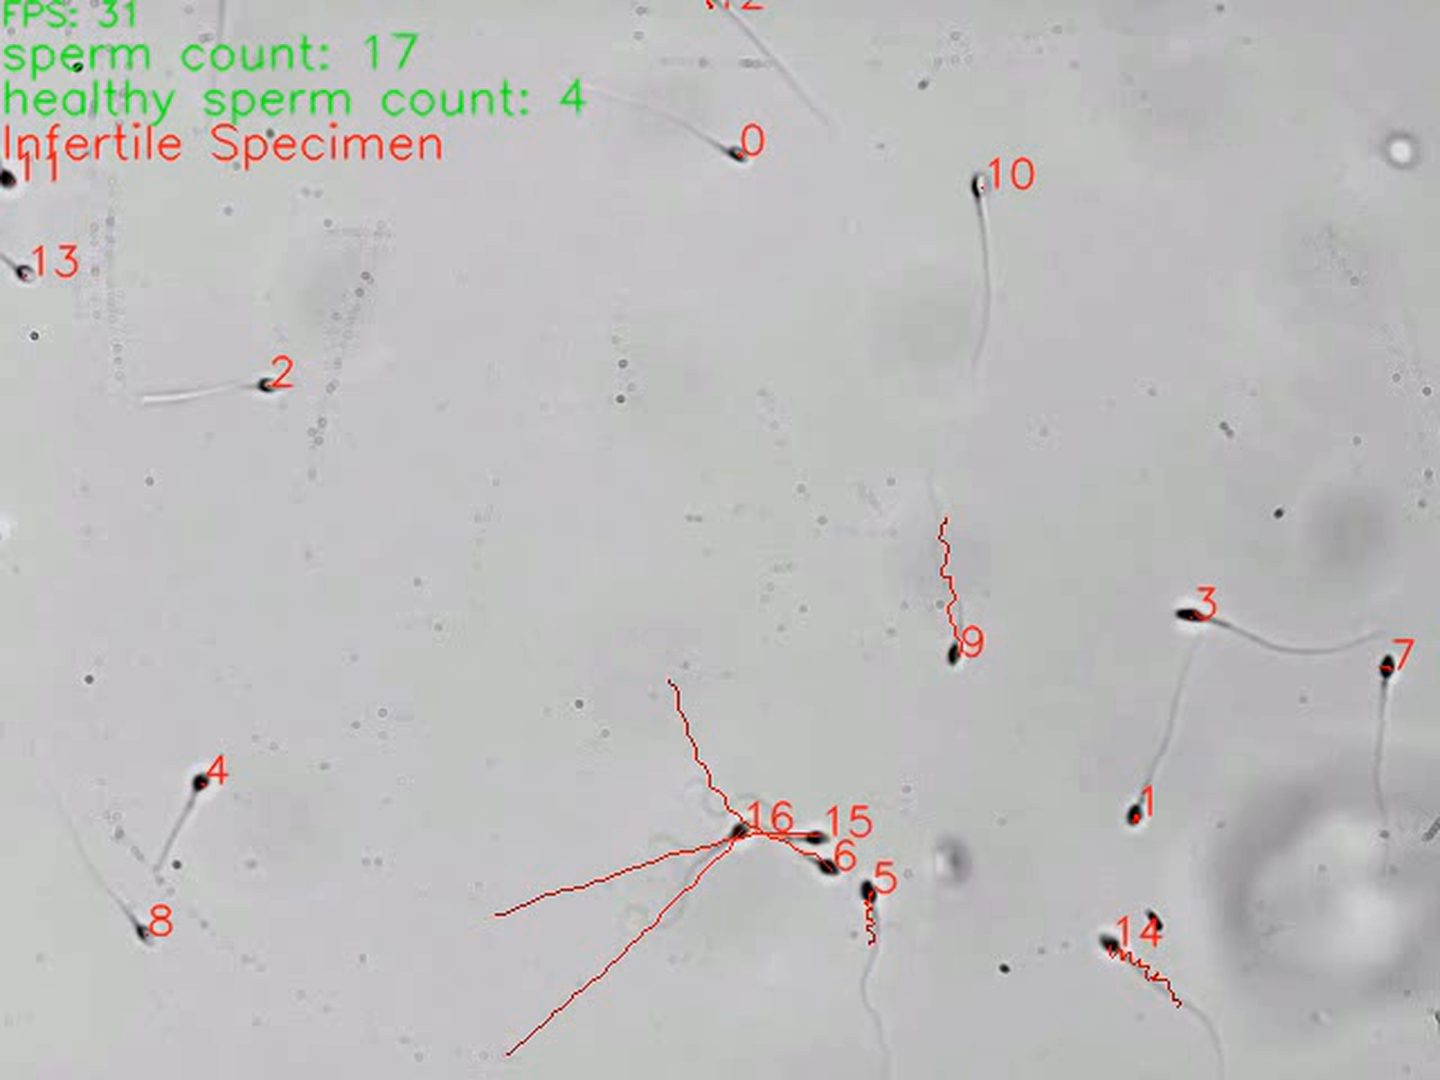
\includegraphics[width=0.75\textwidth]{Images/sam4.png}
    \caption{Sample 4 Output}
    \label{sam4res}
\end{figure}

With clear images, the model's performance was satisfactory. Having relatively fewer sperms, the FPS was well maintained above 30, and the infertility status of the specimen was correctly assessed. Moreover, it dealt with the cross-over of 3 sperms at the same time very well, as shown in Figure \ref{sam4cross}
\begin{figure}[h]
    \centering
    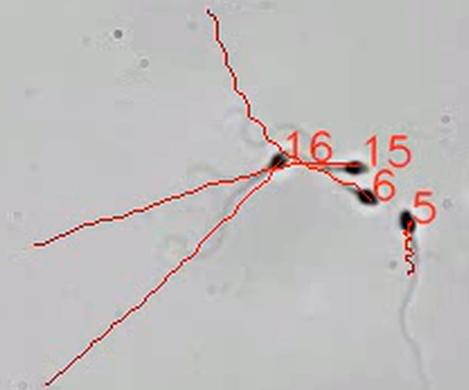
\includegraphics[width=0.42\textwidth]{Images/sam44.png}
    \caption{Cross-Over Tracking of 3 Sperms [IDs: 6, 15, 16] in Sample 4}
    \label{sam4cross}
\end{figure}

\newpage
\subsubsection{Sample 5: Blurry Sperms}
Figure \ref{sam5res} shows the snapshot of the program output of sample 5.
\begin{figure}[h]
    \centering
    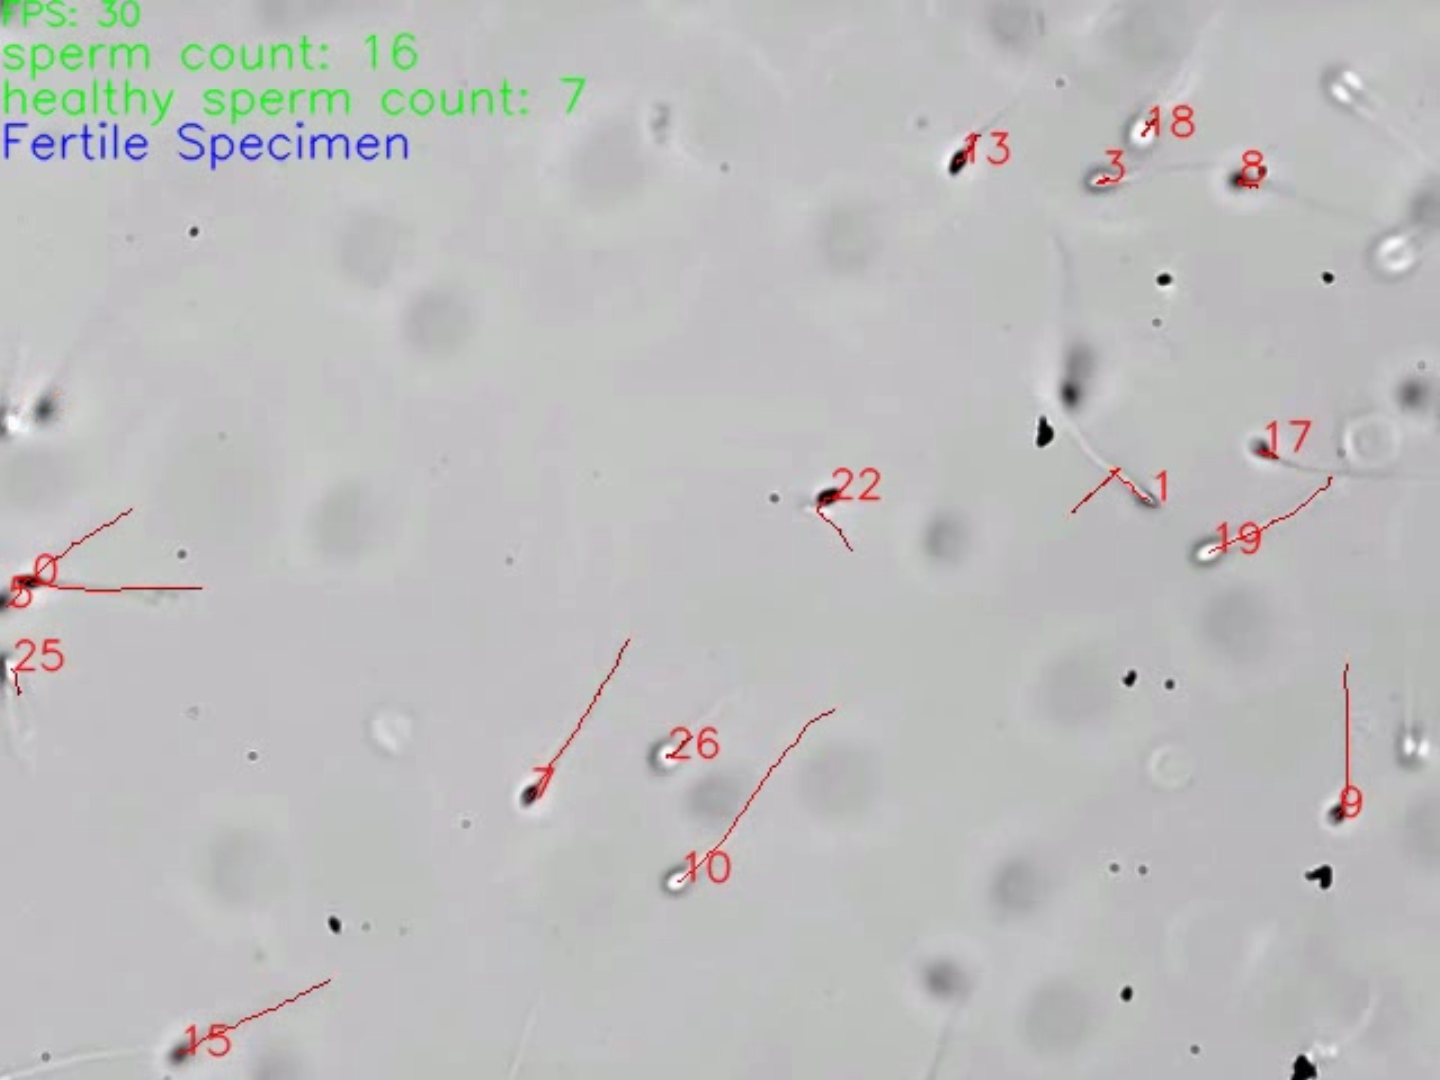
\includegraphics[width=0.75\textwidth]{Images/sam5.png}
    \caption{Sample 5 Output}
    \label{sam5res}
\end{figure}

Even with blurry images, the model still performed quite well. Due to the lower confidence scores, blurry sperms often become undetected from the model and disappear from the video. However, the program keeps track of the sperms even if they are not shown, and the same ID is reassigned to that sperm as soon as the detection is made again. The process can be shown in Figure \ref{sam5keep}.

\begin{figure}[h]
     \centering
     \begin{subfigure}[b]{0.3\textwidth}
         \centering
         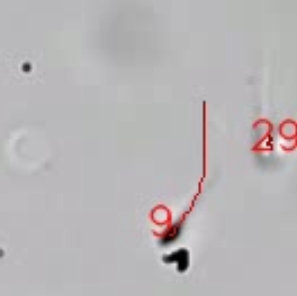
\includegraphics[width=\textwidth]{Images/sam5-4.png}
         \caption{Original Assignment}
     \end{subfigure}
     \hfill
     \begin{subfigure}[b]{0.3\textwidth}
         \centering
         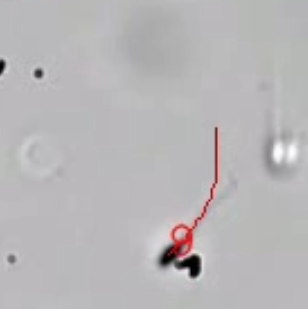
\includegraphics[width=\textwidth]{Images/sam5-5.png}
         \caption{Detection Failure}
     \end{subfigure}
     \hfill
     \begin{subfigure}[b]{0.3\textwidth}
         \centering
         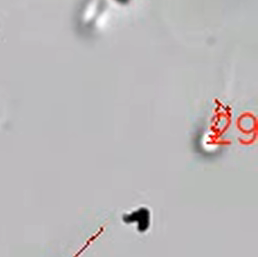
\includegraphics[width=\textwidth]{Images/sam5-6.png}
         \caption{ID Reassigned}
     \end{subfigure}
        \caption{Tracking of Undetected Sperm [ID: 29] in Sample 5}
        \label{sam5keep}
\end{figure}
\newpage
However, there were still a few ID switches, as shown in Figure \ref{sam5switch}.
\begin{figure}[h]
     \centering
     \begin{subfigure}[b]{0.3\textwidth}
         \centering
         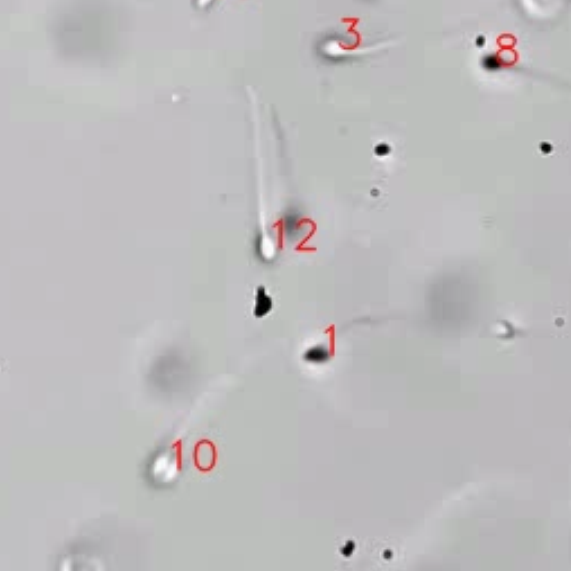
\includegraphics[width=\textwidth]{Images/sam5-1.png}
         \caption{Original Assignment}
     \end{subfigure}
     \hfill
     \begin{subfigure}[b]{0.3\textwidth}
         \centering
         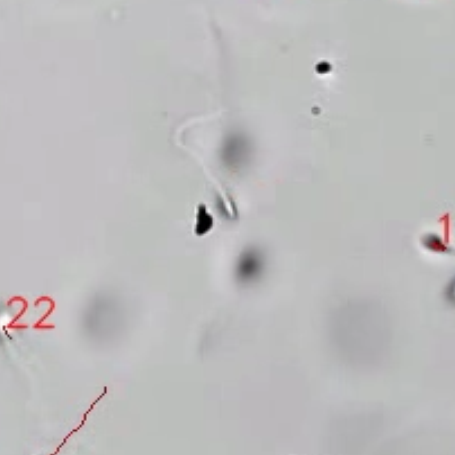
\includegraphics[width=\textwidth]{Images/sam5-2.png}
         \caption{Detection Failure}
     \end{subfigure}
     \hfill
     \begin{subfigure}[b]{0.3\textwidth}
         \centering
         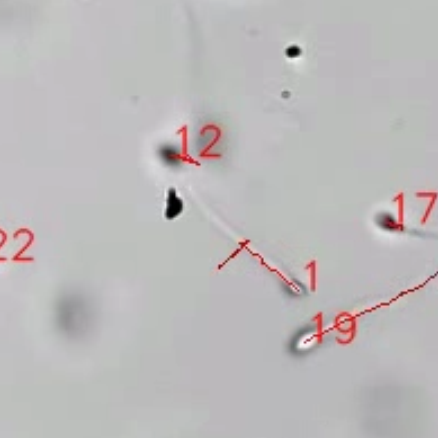
\includegraphics[width=\textwidth]{Images/sam5-3.png}
         \caption{IDs Swapped}
     \end{subfigure}
        \caption{ID Switch [ID: 12, 1] in Sample 5}
        \label{sam5switch}
\end{figure}

This ID switch is due to the short duration of continuous detection of sperm after the initial assignment of ID. The tracking model did not have enough information about the sperms' projected direction. 

This swapping only occurred only once in this sample, and the overall quality of tracking was acceptable. 
\chapter{Future Works}
Although this project successfully completed developing a program that can detect and track sperm cells very well, some limitations and challenges need to be addressed in future work. Some of the main areas of improvement are:

\begin{itemize}
    \item Dataset
    \item Morphology Analysis
    \item Model Optimization
    \item Tracking Performance
    \item Applications
\end{itemize}

\newpage
\section{Dataset}
This program relies on an artificial intelligence detection model trained by the images from the videos provided by the supervising professor. However, the number of images in the current dataset is 1400, which is not a large number by modern standards. Therefore, the model is prone to overfitting and might have lower detection rates when introduced in a new environment. 

Although data augmentation was implemented to mitigate this issue, more data is always better in machine learning if the quality is decent. More data can be collected from different sources and environments. This can improve the detection model's reliability and robustness for real-world applications.

\section{Morphology Analysis}
In this project, only the motility of the sperm was assessed. However, sperm morphology is also essential in assessing sperm quality and fertility because abnormal sperm morphology can affect the sperm's ability to fertilize an egg.

In future work, the detection model will be trained from a multi-class dataset containing the labels of normal and abnormal sperms. The detection model will now be able to detect the location of the sperm as well as the morphological information of the detected sperm. This can provide a more persuasive and practical result for the users of the program.

\section{Model Optimization}
The detection model used in this project is a small-sized version of YOLOv8, a state-of-the-art object detection model. However, there is still room for optimization and improvement. For example, Zhu et al. developed YOLOv5s-SA, a modified version of YOLOv5 with a lightweight structure and enhanced performance. \cite{deep7} By integrating specialized modules for sperm detection into the conventional YOLO model, the performance can be drastically improved. 

Moreover, more effort can be put into optimizing the hyperparameters. In this project, only a few hyperparameters were tuned, whereas YOLOv8 has over 50 tunable hyperparameters. If a sufficient amount of computational resources is provided, the model can further be optimized to its task and have better performance in detecting and tracking.

\section{Tracking Performance}
The tracking algorithm used in this project is based on the Kalman filter. It works well in most cases but still has some limitations and challenges. For instance, the tracking algorithm can lose track of some sperm when they move too fast or occlude each other. Also, the tracking algorithm has less performance when the image is blurry. 

In future work, the tracking performance can be improved using more advanced algorithms or methods. For example, deep learning-based tracking methods can be explored, such as recurrent neural networks (RNN). RNNs specialize in sequential data types, such as text and sound. As videos are also sequences of images, RNNs will also perform well in this field. This method will improve the tracking performance of this program since more flexibility can be expected from deep learning models than traditional algorithmic approaches.

\section{Applications}
This project has demonstrated that a program that detects and tracks sperm cells is feasible and useful. However, many potential applications can be developed based on this program. For example, the program can be integrated with a smartphone app or a web platform to provide real-time feedback and analysis for users who want to test their sperm quality at home. The program can also be used for research purposes to study the effects of different factors on sperm motility and morphology, such as temperature, pH, drugs, etc. The program can also be extended to detect and track other types of cells or microorganisms with similar characteristics to sperm cells.
\chapter{Conclusion}
This project aimed to develop a method for sperm tracking using machine learning and computer vision approaches. The main objectives were to design and build a sperm detection model with YOLOv8 and to utilize the Kalman filter to track the individual sperm to assess motility. The results showed that the proposed method achieved high accuracy and usability. Future work can focus on improving the model performance and versatility by creating a more diverse dataset, adding morphology detection features, enhancing model performance, and developing other applications of this program. 

Many claims that 2023 will be the inflection point for AI development. The increased public interest in popular AI tools, like ChatGPT, has brought more rapid development of other AIs in many fields. Although some are worrying about the rapid development of AI for its unknown effects on society, the emergence of more powerful AI models is inevitable and imminent. As a mechanical engineering student, I did not have any extensive knowledge about AI prior to this project. I am grateful that I was able to study this topic as my final year project before opening a new chapter in my life.
\appendix

\bibliographystyle{ieeetr}
\bibliography{references}

\end{document}
